% =====================================================================
%  Capitolo 6 — Dal brainstorming ai flowchart: come si conduce un
%  brainstorming, flowchart, grafici e matematica di base
%  (problema e soluzione, terza e ultima parte; documentazione visiva)
%  Fonte: trascrizione della lezione GD6 (Game Design, primo anno)
%  Pacchetti richiesti nel preambolo del libro:
%    \usepackage[italian]{babel}, \usepackage[T1]{fontenc},
%    \usepackage[utf8]{inputenc} (solo pdfLaTeX), \usepackage{booktabs},
%    \usepackage{amsmath}, e in più, novità di questo capitolo:
%    \usepackage{tikz} con
%    \usetikzlibrary{shapes.geometric,shapes.symbols,shapes.misc,
%      arrows.meta,positioning,calc,fit}
%    (le librerie vanno caricate nel preambolo, non nel capitolo)
%  Nota sulla fonte: la trascrizione automatica storpia diversi nomi
%  propri (titoli, strumenti, autori) e contiene lunghi tratti ripetuti
%  in loop durante le due pause. Dove il riferimento è ricostruibile con
%  certezza lo si riporta nella forma corretta; dove non lo è, lo si
%  segnala in nota invece di indovinare. Le figure sono ricostruzioni
%  degli esempi mostrati a lezione (slide e lavagna draw.io), non copie.
% =====================================================================

\chapter[Dal brainstorming ai flowchart]{Dal brainstorming ai flowchart:
condurre un brainstorming, flowchart, grafici e matematica di base}
\label{cap:brainstorming-flowchart}

Con questo sesto capitolo si chiude, finalmente, la lunga lezione su
\emph{problema e soluzione} cominciata due capitoli fa
(capitolo~\ref{cap:problema-soluzione}) e proseguita nel precedente
(capitolo~\ref{cap:ricerca-idee}). Mancava l'ultima parte: \emph{come} si
conduce un brainstorming, con quali regole, quali tecniche e come si passa
da cento idee a una manciata di idee valutate. Chiusa quella, la giornata
cambia argomento e apre un blocco nuovo, dedicato agli strumenti
\textbf{visivi} della documentazione: i \textbf{flowchart}, i
\textbf{grafici} e quel poco di \textbf{matematica di base} che serve per
costruirli e leggerli.

La lezione, un venerdì pomeriggio a ridosso di Halloween, si tiene da remoto
ed è condotta ancora da Mattia Podini. Il percorso del capitolo ne ricalca la
struttura:
\begin{enumerate}
  \item le domande in apertura, ancora una volta sul \textbf{production
        dictionary} di Pokémon: che cosa si intende per
        \emph{nomenclatura}, come ordinare le voci, che cosa lasciare ad
        altri documenti (sezione~\ref{sec:pd-gd6});
  \item la conclusione della parte sul \textbf{brainstorming}: le condizioni
        per farlo bene, il \textbf{facilitatore}, le pause e il cibo
        (sezioni~\ref{sec:ripresa-gd6} e~\ref{sec:condurre-brainstorming});
  \item altre \textbf{tecniche} per generare idee, dai \emph{sei cappelli} al
        \textbf{TRIZ}, le regole dell'innovazione di \textbf{Guy Kawasaki} e lo
        \textbf{SCAMPER} (sezioni~\ref{sec:altre-tecniche}
        e~\ref{sec:kawasaki-scamper});
  \item come si passa \textbf{dalle cento alle dieci idee}: la
        \emph{brainstorming matrix}, il confronto, il tentativo di
        distruggere le proprie idee, il prototipo e le routine da spezzare
        (sezioni~\ref{sec:sortare-idee} e~\ref{sec:kiss-routine});
  \item i \textbf{flowchart}: che cosa sono, dove nascono, a che cosa servono
        a un designer, le regole di lettura, i blocchi, l'obbligo di chiudere
        il flusso, e una serie di esempi reali che le regole le piegano
        (sezioni~\ref{sec:flowchart-cosa}--\ref{sec:flowchart-esempi});
  \item il task della settimana: il \textbf{flowchart completo di Pac-Man}
        (sezione~\ref{sec:task-gd6});
  \item i \textbf{grafici}: un piccolo esercizio in aula (linea o gradini?),
        i grafici di base, quelli più ricchi e la mappa della campagna di
        Russia di Napoleone, ``uno dei grafici più belli mai fatti''
        (sezioni~\ref{sec:grafici-esercizio}--\ref{sec:principi-grafici});
  \item la \textbf{matematica di base}: media, media pesata, proporzioni
        (sezione~\ref{sec:matematica-base}).
\end{enumerate}

% ---------------------------------------------------------------------
\section{In apertura: ancora il production dictionary}
\label{sec:pd-gd6}

\subsection{Prima di cominciare}

L'avvio è il solito avvio di una lezione online: il docente non sente la
classe (``probabilmente perché non ho ancora condiviso lo schermo''), segna le
presenze, saluta chi entra. Poi il rituale: domande o dubbi sulla lezione
precedente, che oggi si conclude, o sui task in generale, ``anche perché il
production dictionary scade lunedì'' (il task del
capitolo~\ref{cap:problema-soluzione}, sezione~\ref{sec:task-gd4}).

\paragraph{Problemi di gameplay, prima di tutto.} La prima domanda riguarda
invece il task a gruppi sui \emph{pain point}
(sezione~\ref{sec:task-gd5}): i tre problemi principali trovati devono
riguardare il gameplay o possono toccare qualsiasi feature del gioco, per
esempio il negozio? Qualsiasi tipo di feature, chiaramente. Il docente però
\textbf{sconsiglia} di prendere un problema \textbf{artistico} o un problema
di \textbf{performance}: se davvero non si trova altro, lo si può includere
come punto finale, ma la priorità va ai \textbf{problemi di gameplay}.

\subsection{Che cosa si intende per nomenclatura}

Mattia, uno studente, confessa di non aver ancora capito la consegna del
production dictionary. Ha provato a lavorarci in una cartella personale, ma
si è accorto che stava scrivendo e \emph{spiegando meccaniche}, e ha il
sospetto che non sia quello che viene chiesto. ``Che cosa si intende per
nomenclatura?''

Il docente ricorda di averlo già ripreso all'inizio della lezione precedente
(sezione~\ref{sec:pd-ripreso}) e lo rispiega. L'obiettivo è spiegare
\textbf{nomi unici legati al gioco}, o alla produzione del gioco. Possono
essere nomi di meccaniche, e nel caso di Pokémon lo possono essere
tranquillamente; ma più spesso sono nomi che spiegano un oggetto del mondo,
un \emph{game object} del mondo di Pokémon. L'esempio è il \textbf{tipo} (o
elemento): si spiega che cosa sono i vari tipi, che cos'è il tipo di un
Pokémon.

\paragraph{Che cosa \emph{non} ci va.} Negli esempi mostrati nelle slide,
come la voce \emph{Chase} (lo stato di inseguimento di un'intelligenza
artificiale, sezione~\ref{sec:production-dictionary}), è chiaro che quello
stato non verrà spiegato in un documento dedicato solo a lui: sarà spiegato
nel documento delle IA. Lì si trovano le spiegazioni \textbf{profonde}: come
funziona la meccanica, che parametri ha, che cosa richiede lato
programmazione, lato arte e così via. Nel production dictionary finisce
invece \textbf{a che cosa è legato quel nome}, a livello descrittivo: una o
due righe, una descrizione succinta. Lo scopo è che il lettore, di qualunque
natura sia (artista, grafico, programmatore, designer), sappia \textbf{a che
cosa si riferisce quella parola}.

\paragraph{La webcam, per favore.} A metà spiegazione il docente chiede a
Mattia di accendere la webcam: ``già faccio fatica a leggere naturalmente i
volti delle persone, figuriamoci se non ti vedo''; vuole capire se la
spiegazione arriva o no. Il problema dello studente era proprio questo:
quando si metteva a scrivere, gli veniva spontaneo descrivere le meccaniche,
non le nomenclature.

\subsection{Priorità: un limite di una pagina}

Per tutto ciò che è estremamente specifico si fa riferimento ai
\textbf{singoli documenti}. E gli studenti hanno anche il limite di
\textbf{una pagina}, quindi devono per forza scegliere le nomenclature
\textbf{più importanti} del gioco. Con molto più spazio si potrebbe discutere
se spiegare meccaniche uniche, specifiche, o qualcosa di estremamente
laterale.

\paragraph{Un caso limite.} Spiegare una singola mossa molto particolare è un
caso estremamente unico,\footnote{Nella trascrizione la mossa compare come
``fuoco-bomba''; non è chiaro a quale mossa o meccanica ci si riferisca.
L'esempio vale comunque come caso estremamente specifico.} ben diverso dallo
spiegare, per esempio, che cos'è una \textbf{MT} o una \textbf{MN}. E anche
per le MT conviene separare due piani:
\begin{itemize}
  \item \textbf{come funziona il sistema}: se una MT è consumabile o no,
        quante mosse ci sono e così via; questo può essere relegato ad altra
        documentazione;
  \item \textbf{che cos'è}: questo sì, è materia da dizionario.
\end{itemize}
Ancora più a monte si potrebbe spiegare che cos'è un \emph{oggetto} di gioco,
un item della borsa; ma ``oggetto'' è abbastanza comprensibile. L'ultima
parola spetta agli studenti, ma il criterio del docente è questo: si parla di
\textbf{nature uniche del gioco}, oppure \textbf{fraintendibili}. È questa
l'utilità del documento.

\paragraph{Non è un errore, è un'altra scelta.} Quello che allo studente
veniva istintivamente da fare non è sbagliato di per sé: rispetto alla
consegna è un'altra cosa, ma dal punto di vista della produzione non è un
errore. Come detto l'ultima volta, il production dictionary si può
\textbf{ibridare} con altri documenti (sezione~\ref{sec:pd-ripreso}): lo si
può mettere all'inizio di un documento, oppure spiegare le singole
terminologie in un GDD o in un altro tipo di documentazione, e allora quello
è il documento che spiega quella meccanica. Se il gioco \textbf{non ha un
grande rischio di fraintendimento}, si può anche valutare di avere un
documento a sé che funge da dizionario: non è obbligatorio.

\subsection{Raggruppare o ordinare alfabeticamente?}

Intanto Lorenzo ha la webcam spenta: ``vedo che Lorenzo si è affondato
nell'erba alta ed è diventato un Pokémon''. La parola passa a Valerio, che
ha stilato una serie di elementi e, siccome erano tanti, li ha
\textbf{raggruppati per fili comuni}. È sbagliato?

Dipende dal numero, dalla mole di informazioni che si danno al lettore. Su
una pagina sola può funzionare; quale sia la scelta ideale il docente non
può dirlo (``sennò poi dopo me la modificate''). Ma il ragionamento è
questo, esattamente come per un dizionario:
\begin{itemize}
  \item la \textbf{maggior leggibilità}, nel vuoto, ce l'ha l'\textbf{ordine
        alfabetico};
  \item l'ordine alfabetico però non risolve un problema: alcune
        nomenclature sono \textbf{legate ad altre}. L'esempio, forse un
        azzardo, è \emph{Pokémon} e \emph{Poké Ball}: al lettore potrebbe
        essere utile sapere prima l'informazione più rilevante e subito
        dopo quella associata.
\end{itemize}
Nel caso degli studenti può contare meno; in production dictionary
esageratamente grossi conta di più. In ogni caso, se il production dictionary
c'è (e non è una necessità averlo nella produzione), \textbf{deve essere
ordinato}.

\paragraph{I problemi di stato.} Valerio ha anche parlato delle lotte,
elencando e descrivendo tutti i \textbf{problemi di stato}: dovrebbero stare
in un documento a parte, dedicato alle lotte? ``Posso fare un esempio?''
``Certo che puoi farlo, però io poi sarò libero di non risponderti.'' È più
un problema di \textbf{priorità sulle nomenclature}; sul fatto di avere un
documento a parte o meno, il docente preferisce non rispondere adesso: se ne
riparlerà dopo che avrà commentato il documento.

Una piccola nota di colore chiude il giro: Mattia non sa come abbassare la
mano su Zoom. ``Non sono lo Zoom guru, quindi figurati.''

% ---------------------------------------------------------------------
\section{Dove eravamo rimasti}
\label{sec:ripresa-gd6}

\subsection{La forbice che si allarga}

Se non c'è altro, si conclude la lezione su problema, idea, ricerca e
brainstorming. L'ultima volta ci si era fermati quasi alla fine: manca
la parte sulle \textbf{metodologie per fare brainstorming}.

Il docente ricorda una cosa che vale per tutta la lezione: più si va avanti,
dall'inizio verso la fine, più \textbf{la forbice si amplia}.
\begin{description}
  \item[Nella ricerca] non ci sono limiti, ma c'è almeno una struttura: una
        forma dei dati, delle priorità (target audience, competitor e così
        via). Dare priorità è soprattutto una questione di
        \textbf{tempistiche}: in pre-produzione il tempo sarà poco e ci sarà
        tanto da fare, quindi quanto più si riesce a coprire di quella lista
        non omnicomprensiva (la mappa della ricerca,
        sezione~\ref{sec:mappa-ricerca}), meglio è. Alcune cose andrebbero
        fatte subito: i \textbf{competitor}, fondamentali, e
        l'\textbf{utente}, più di tutti; anche il \textbf{mercato} è
        importante. Le priorità ci saranno per forza, perché il tempo non è
        infinito. E per la ricerca strutture e framework ce ne sono, e sono
        abbastanza codificati: la lista vista (le Liberating Structures),
        la SWOT analysis, la perceptual mapping
        (sezione~\ref{sec:perceptual-mapping}).\footnote{Nella trascrizione
        compaiono come ``la lista di pesciola'' (verosimilmente un
        riferimento storpiato alla lista delle Liberating Structures,
        sezione~\ref{sec:problema-necessita}) e ``swap analysis'', che è
        quasi certamente la SWOT analysis (\emph{Strengths, Weaknesses,
        Opportunities, Threats}).}
  \item[Nell'ideazione] e nel brainstorming le tecniche ci sono, ma il campo
        è \textbf{probabilmente infinito}. Si può adottare più o meno
        quello che si vuole, soprattutto a seconda del gruppo che fa
        brainstorming: non è detto che ci sia l'intero team, magari solo il
        team di design, o un \emph{feature team} all'interno del team di
        design. A seconda di chi si è nel team e di quanto è grande, si può
        davvero fare quello che si vuole: ``potete giocare a freccette,
        far venire in mente le idee, o giocare a biliardo, davvero
        qualsiasi cosa funziona''.
\end{description}
Va bene tutto, \textbf{fintanto che porta un risultato}: quella
``fantomatica'' ideazione di \textbf{cento idee} da \emph{sortare} e scartare
(sezione~\ref{sec:principi-brainstorming}).

% ---------------------------------------------------------------------
\section{Come si conduce un brainstorming}
\label{sec:condurre-brainstorming}

\subsection{Le condizioni}

Ci sono però alcune condizioni importanti.

\paragraph{Nessuno viene fermato.} Durante il brainstorming, cioè nel momento
in cui si generano le idee, \textbf{nessuno deve essere fermato} dal
generarle. Non si scartano subito potenziali idee che ``non c'entrano
nulla'': \textbf{le si elenca tutte}. Poi, eventualmente, ci sarà una fase,
insieme o da soli, in cui queste idee vengono \textbf{filtrate}.

\paragraph{Tutti devono poter parlare.} Tutti devono sentirsi nella
condizione di dire la propria e di far crescere quella grande lista di idee,
che alla fine dei conti è l'obiettivo: buttare giù davvero qualsiasi cosa.
Anche perché quello che verrà scartato può ritornare in un'altra forma, in
un'altra maniera, o anche solo far scaturire qualche idea nuova per
implementazioni future. Qualsiasi spunto è utile: lasciare la parola a
tutti, e nella fase di brainstorming \textbf{qualsiasi cosa va bene}.

\paragraph{Non solo designer.} Sempre per arrivare a una quantità maggiore,
e potenzialmente più \textbf{diversificata}, di idee, conviene avere nel
brainstorming \textbf{non solo designer}, o comunque non solo persone con lo
stesso background. A seconda di quanto sono disponibili e di quanto sono
dentro l'industria, si cercano \textbf{punti di vista diversi}: l'obiettivo è
ampliare la propria visione il più possibile.

\subsection{Il facilitatore}

Questo vale sicuramente per i team grossi, ma va valutato anche per quelli
piccoli, soprattutto le prime volte, se c'è difficoltà a parlare o se si è
meno portati a rompere il ghiaccio o a essere espansivi: conviene avere un
\textbf{facilitatore}. Non un leader, ma qualcuno che si preoccupa di
\textbf{controllare il flusso} del brainstorming: quanto tempo si sta
spendendo a discutere di un'idea, o ``a tirare quella freccetta''.

Il facilitatore ha fondamentalmente \textbf{due obiettivi}:
\begin{enumerate}
  \item \textbf{assicurarsi che tutti stiano bene} durante il brainstorming.
        A livello pratico vuol dire che tutti parlino e abbiano lo stesso
        tempo per parlare; ma c'è un passo in più, che tutti si sentano
        \textbf{a proprio agio}. Garantire la parola a tutti non basta
        necessariamente: a seconda dei membri del team, e di quanto li si
        conosce, l'obiettivo è \textbf{farli sentire ascoltati};
  \item \textbf{assicurarsi che il brainstorming abbia uno scopo pratico}.
        Fare brainstorming ``è una figata, piace a tutti'', ma il rischio
        di ``buttarla in caciara'' è molto grosso. È bello avere un momento
        di comunione con il team, più o meno regolamentato; tuttavia
        \textbf{bisogna quagliare}, arrivare a una lista lunga e concreta di
        idee. Il facilitatore si chiede quanto tempo va dedicato al
        brainstorming (un'ora?), controlla che si stia andando nella
        direzione corretta ed eventualmente \textbf{tira le redini} se
        qualcuno sta divagando.
\end{enumerate}

\paragraph{Approfondimento: chi deraglia, rimette sui binari.} Schell, tra i
suoi sedici consigli pratici per il brainstorming (\emph{The Art of Game
Design}, capitolo~7), incoraggia a \textbf{fare battute}: le battute
sciolgono la mente e fanno vedere le cose da prospettive che si erano perse,
ed è dalle prospettive nuove che nascono le grandi idee. Ma avverte che,
soprattutto in gruppo, le battute possono portare fuori strada; uscire dai
binari ogni tanto va bene (``le idee buone potrebbero non essere sui
binari''), purché ci si prenda la responsabilità di rientrarci. Il suo
comandamento è: \emph{he who derails, rerails}, chi fa deragliare rimette sui
binari. È, in piccolo, il secondo compito del facilitatore distribuito su
tutti i partecipanti.

\subsection{Pause e cibo}

\paragraph{Fare delle pause.} Conviene avere \textbf{pause tra una fase e
l'altra}. Al secondo anno si parlerà meglio di come affrontare la produzione,
di come lavorare con altri esseri umani, dell'importanza delle soft skill;
cose importanti, che il docente non vuole sminuire, ma il primo anno è il
campo di prova. Le pause servono a ridurre ``il cortisolo, mettiamola
così'': evitare che le persone impazziscano o che comincino a percepirsi
\textbf{screzi} forti tra gli individui.

È il discorso precedente visto dall'altro lato: se non si fa parlare tutti,
e soprattutto se qualcuno comincia a \textbf{smontare le idee}, o fa già la
fase di prendere un'idea e buttarla subito fuori dal cesto perché non ha
senso con i limiti, con la visione o con quello che si vuole, qualcuno
potrebbe ``inalberarsi'', prenderla male. E si ammetta pure che il team sia
grosso e che ci siano già delle inimicizie al suo interno.

\paragraph{Portate il cibo.} Per risolvere questo problema: pause, e poi
\textbf{cibo}. Lo si vedrà in modo più strutturato al secondo anno, ma il
mantra è: ``portate il cibo, portate la pizza. Non lo so, quello che
mangiano gli esseri umani generici. Io non mangio la pizza, però\dots''.
Generalmente avere delle pause in cui si mangia e si beve \textbf{aiuta
notevolmente a ridurre la tensione}.

% ---------------------------------------------------------------------
\section{Altre tecniche per generare idee}
\label{sec:altre-tecniche}

\subsection{Una lista, non un programma}

I modi per fare brainstorming, per generare idee in generale, sono tanti. Il
docente non li vede tutti punto per punto, ma li elenca; si aggiungono a
quelli già visti nel capitolo precedente (sezione~\ref{sec:tecniche-idee}).

\subsection{Circle}

Ci si mette \textbf{in cerchio}, si scrive una parola, si va avanti. Si
comincia con, per esempio, il tipo di gioco, una \emph{game quality}, un tema,
un'emozione; si passa il foglietto alla persona successiva, che aggiunge
un'altra parola, e così via finché il giro non è finito. A volte si fanno
più giri. È un modo per \textbf{ibridare la propria idea iniziale con
quelle degli altri} e vedere che cosa esce.\footnote{Il docente lo associa,
``se non sbaglio'', a un gioco dei futuristi. Il meccanismo descritto
(ciascuno aggiunge un pezzo senza controllare l'insieme) ricorda piuttosto il
\emph{cadavre exquis} dei surrealisti.}

\subsection{Acting brainstorming}

Si \textbf{mette nei panni di un'altra persona}: nella slide, una persona
famosa, un personaggio famoso. Ma vale anche, più in generale, per mettersi
nei panni di qualcun altro: avere la capacità \textbf{empatica} di vedere come
si è percepiti dall'altra parte, o che cosa si potrebbe provare dall'altra
parte.

\paragraph{Fuori dal brainstorming.} Il concetto è utile ben oltre la fase di
brainstorming. Un esempio: un 3D artist o un concept artist consegna i suoi
concept e gli vengono rimandati indietro, ogni volta, per una determinata
ragione. È ovvio, o almeno molto probabile, che il suo \textbf{morale} si
riduca. Mettersi nei suoi panni aiuta; poi bisognerà capire perché succede e
come risolverlo. Mettersi nei panni dell'altro aiuta a spiegare alcune
problematiche della produzione e del team: il morale basso, una persona che
non è mai presente o che non parla mai durante i meeting. Come sempre, si
cerca di arrivare alla \textbf{radice del problema}
(sezione~\ref{sec:problema-necessita}).

\subsection{I sei cappelli}

I \textbf{sei cappelli} vengono da un libro\footnote{\emph{Six Thinking Hats}
di Edward de Bono (1985), noto in italiano come \emph{Sei cappelli per
pensare}.} e possono essere utili per diversi tipi di attività. Ogni cappello
ha una \textbf{durata specifica} a seconda dell'attività ed è associato, un
po' come nell'acting brainstorming, alla necessità di guardare o di agire da
un determinato punto di vista:
\begin{description}
  \item[Blu] la \emph{big picture}: si guarda il problema ad alto livello;
  \item[Bianco] fatti e informazioni: si guardano i fatti, i dati;
  \item[Rosso] più istintivo: \emph{feelings and emotions};
  \item[Nero] il \textbf{giudizio critico}. Questo \textbf{rompe la fase di
        brainstorming}: è utile quando si comincia già a \emph{sortare} le
        idee, ``senza ciarle'';
  \item[Giallo] estremamente positivo: ``yes'', sorriso ``a 34 denti'', si va
        avanti;
  \item[Verde] le \textbf{idee nuove}.
\end{description}
È chiaro quindi che la fase di brainstorming dovrebbe partire col
\textbf{verde}, e comunque avere tanti momenti ``col cappello verde''. A volte
si passa da una fase all'altra; la lista completa è nel libro, che non è
necessario leggere, ma si trova anche in giro.

\subsection{L'oggetto dal cappello}

``Questo piace particolarmente a Diego'', il direttore del corso, e serve a
mostrare ancora una volta che nel generare idee si può infilare dentro
qualsiasi cosa. Si sfruttano \textbf{oggetti particolari, gadget}, pescati da
un ``fantomatico'' cappello, e si fa brainstorming su quell'oggetto: che cosa
c'entra, e come può aiutare a risolvere il problema. ``Utile? Non lo so, io
non l'ho mai usato, però sta qua.''

\paragraph{Approfondimento: i giocattoli sul tavolo.} Schell propone qualcosa
di molto simile tra i suoi consigli per il brainstorming
(\emph{The Art of Game Design}, capitolo~7, \emph{Toys}): portare al tavolo
dei giocattoli, alcuni legati al problema e altri che non c'entrano niente.
Il suo paragone sono i ristoranti pieni di oggetti strani alle pareti: non
sono decorazione, sono spunti di conversazione. I giocattoli coinvolgono la
creatività anche in modo \textbf{tattile}; e se si porta un po' di
plastilina per modellare le idee, ``sembra stupido, ma la creatività è
stupida''.

\subsection{Storyboard}

Lo \textbf{storyboard} è un po' come il \emph{drawing}
(sezione~\ref{sec:tecniche-idee}): non importa saper disegnare bene o male,
importa che sia \textbf{chiaro}, anche con gli stickman. Si disegna il
processo, una potenziale storia che spieghi l'idea, che la ``metta a terra''
nel brainstorming.

\subsection{Le domande}

\textbf{Domande}: ci si butta dentro più domande possibili, su qualsiasi
cosa. È anche un modo, più o meno serio, per iniziare quel tipo di
``sortaggio'' (``non sorteggio, sortaggio''), cioè di \textbf{valutazione}
delle idee messe a terra.

\subsection{Papà e mamma: peggiore è, meglio è}

Un'altra tecnica importante è presentata nelle slide con una metafora
familiare: da una parte il \emph{papà}, la figura particolarmente
\textbf{pragmatica}; dall'altra la parte in cui ci si butta dentro davvero
qualsiasi cosa e va bene. Anzi: \textbf{peggiore è l'idea, meglio è},
almeno teoricamente. Sempre nell'idea che \textbf{tutto può aiutare}, e che
la soluzione si può trovare partendo da qualsiasi cosa.\footnote{La
trascrizione non permette di ricostruire con certezza il nome della tecnica
nella slide. L'impostazione (cercare deliberatamente le idee peggiori) è
quella nota come \emph{worst possible idea} o \emph{reverse brainstorming}.}

\paragraph{Approfondimento: scrivere tutto, anche le idee stupide.} Schell
(\emph{The Art of Game Design}, capitolo~7, \emph{Write Everything}) cita
Linus Pauling: ``il modo migliore per avere una buona idea è avere molte
idee''. Il suo consiglio è di non aspettare l'idea brillante ma di scrivere
\textbf{tutto} ciò che è anche solo lontanamente collegato al problema, ogni
idea stupida che passa per la testa: bisogna far uscire quelle stupide prima
che comincino ad arrivare quelle buone, e a volte un'idea stupida diventa
l'ispirazione per un'idea geniale. Non ci si censura, e soprattutto in
gruppo non si censurano gli altri: ``le loro idee stupide valgono quanto le
tue''.

\subsection{Associative e mind mapping}

Con l'\textbf{associative} si parte da una parola e le si associano parole
simili. Si può usare anche un \emph{word association tool}, un'IA o
qualsiasi software che associa parole.

È molto simile al \textbf{mind mapping}, che si vede di solito: ``sicuramente
l'avrete vista da qualche parte''. Quando si parla di brainstorming, la
visione pratica è generalmente questa: una \textbf{grande mappa sulla
lavagna}, che tutti devono poter vedere. Si parte da un concetto, si
dividono i rami per \textbf{categorie}, e i rami grossi portano a rami più
piccoli, con parole o concetti sempre legati alla categoria principale
(figura~\ref{fig:mind-map}).

\begin{figure}[htbp]
\centering
\begin{tikzpicture}[
    font=\small,
    centro/.style={ellipse, draw, thick, minimum width=2.6cm,
                   minimum height=1cm, align=center},
    ramo/.style={rectangle, rounded corners=3pt, draw, align=center,
                 minimum height=0.7cm, inner sep=4pt},
    foglia/.style={align=center, inner sep=2pt, font=\footnotesize},
    every edge/.style={draw}]
  \node[centro] (c) {Gioco sul\\viaggio nel tempo};
  \node[ramo] (m) at (-4.2,1.6) {Meccaniche};
  \node[ramo] (t) at (4.2,1.6) {Tema};
  \node[ramo] (e) at (-4.2,-1.6) {Emozioni};
  \node[ramo] (p) at (4.2,-1.6) {Pubblico};
  \draw[thick] (c) -- (m); \draw[thick] (c) -- (t);
  \draw[thick] (c) -- (e); \draw[thick] (c) -- (p);
  \node[foglia] (m1) at (-6.3,2.6) {riavvolgere};
  \node[foglia] (m2) at (-6.4,1.0) {loop};
  \node[foglia] (m3) at (-3.0,2.7) {paradosso};
  \draw (m) -- (m1); \draw (m) -- (m2); \draw (m) -- (m3);
  \node[foglia] (t1) at (6.3,2.6) {orologi};
  \node[foglia] (t2) at (6.4,1.0) {rovine};
  \node[foglia] (t3) at (3.0,2.7) {nostalgia};
  \draw (t) -- (t1); \draw (t) -- (t2); \draw (t) -- (t3);
  \node[foglia] (e1) at (-6.3,-2.6) {rimpianto};
  \node[foglia] (e2) at (-6.4,-1.0) {sorpresa};
  \node[foglia] (e3) at (-3.0,-2.7) {ansia};
  \draw (e) -- (e1); \draw (e) -- (e2); \draw (e) -- (e3);
  \node[foglia] (p1) at (6.3,-2.6) {puzzle lover};
  \node[foglia] (p2) at (6.4,-1.0) {sessioni brevi};
  \node[foglia] (p3) at (3.0,-2.7) {mobile};
  \draw (p) -- (p1); \draw (p) -- (p2); \draw (p) -- (p3);
\end{tikzpicture}
\caption{Struttura tipica di una mind map: un concetto centrale, rami
principali per categoria e rami secondari sempre legati alla categoria da
cui partono. Il contenuto è un esempio inventato.}
\label{fig:mind-map}
\end{figure}

\paragraph{Che cosa usare per il task.} Per il task in corso
(sezione~\ref{sec:task-gd5}) il mind mapping funziona molto bene, ma possono
funzionare anche l'associative o il circle. Questi, i più
\textbf{immediati}, sono quelli che il docente consiglia al momento.

\paragraph{Approfondimento: lo spazio ricorda.} Due consigli di Schell
(\emph{The Art of Game Design}, capitolo~7) spiegano perché la mappa sulla
lavagna funziona. Il primo (\emph{The Writing on the Wall}): in gruppo serve
una superficie che tutti vedano contemporaneamente; Schell preferisce grandi
fogli adesivi o carta da pacchi alle pareti, che si possono riposizionare,
staccare, arrotolare e conservare, per riprendere un anno dopo il
brainstorming ``come se non si fosse mai interrotto''. Il secondo
(\emph{The Space Remembers}, espressione presa da Tom Kelley): la memoria per
le liste è scarsa, ma quella per la \textbf{posizione} delle cose intorno a
noi è ottima; appendere le idee nella stanza aiuta a ritrovarle e a vederne
le connessioni. Un terzo consiglio è più sorprendente
(\emph{Number Your Lists}): \textbf{numerare} le liste le rende più facili da
discutere (``mi piacciono dalla 3 alla 7'') e, stranamente, dà alle voci una
certa dignità, così che vengono prese più sul serio.

\subsection{TRIZ}
\label{sec:triz}

Il \textbf{TRIZ}, già accennato (sezione~\ref{sec:tecniche-idee}), viene
solo ``accennato'' anche qui, perché è estremamente complesso. Nasce
nell'\textbf{Unione Sovietica}. Il concetto è un po' quello dell'astrazione
vista nel SIT, il \emph{closed world}: il problema, per come viene
formulato, contiene già la soluzione. Anzi, \textbf{non trovare la soluzione
dipende dal fatto che il problema non è formulato correttamente}. La
soluzione è già lì; per arrivarci bisogna \textbf{astrarre il problema},
trovare \textbf{soluzioni astratte} e poi \textbf{concretizzarle}. ``Questo è
il salto.''

\paragraph{Come funziona.} Il TRIZ nasce dall'analisi di un numero enorme di
\textbf{brevetti} sovietici, in cui il comune denominatore era astrarre i
problemi e vedere come erano stati risolti. Problemi e soluzioni vengono
messi in una \textbf{matrice} con righe e colonne: sulle righe e sulle
colonne ci sono le stesse \emph{feature}, da 1 a $n$ (``sono 40, se non
sbaglio, forse sono state anche aumentate nel
tempo'').\footnote{Nella formulazione classica di Genrich Altshuller la
\emph{matrice delle contraddizioni} incrocia 39 parametri tecnici (righe:
il parametro che si vuole migliorare; colonne: quello che peggiora di
conseguenza), e ogni cella suggerisce alcuni dei \textbf{40 principi
inventivi}. Versioni successive (come la \emph{Matrix 2003}) hanno esteso i
parametri. Nella trascrizione il nome compare come ``Drizzt'', ``TRIPS'' e
``TRIZZE''.} Le feature possono essere il peso di un oggetto in movimento,
il peso di un oggetto stazionario, la lunghezza di un oggetto in movimento,
la lunghezza di uno stazionario, l'area di un oggetto in movimento, e così
via.

Se si riesce ad astrarre il proprio problema e a trovare la riga e la
colonna su cui si fonda, si va a cercare la \textbf{cella} che le combina.
Un esempio: il problema è mantenere caldo il contenuto di un bicchiere
\textbf{senza far scottare le mani} di chi lo tiene. Il calore fa parte di
quel tipo di feature: si cerca la cella che combina la colonna e la riga del
problema.

\paragraph{Piegarsi alle regole.} Il TRIZ si basa principalmente su
\textbf{problemi meccanici}, e non è facile. La soluzione, se si usa il TRIZ,
\textbf{deve derivare da quello che viene consigliato nella cella}: per
usarlo non basta conoscerlo, bisogna anche piegarsi alle sue regole. Può
essere un buon modo, se ci si leggono righe e colonne, soprattutto per
\textbf{problemi pratici di produzione fisica}: per esempio nei giochi da
tavolo, dove la stampa, la grandezza o il costo di una componente è
eccessivo. Ma resta estremamente codificato: è tra le cose che si possono
approfondire.

% ---------------------------------------------------------------------
\section{Le regole di Kawasaki e lo SCAMPER}
\label{sec:kawasaki-scamper}

\subsection{Le regole dell'innovazione di Guy Kawasaki}

Le \textbf{regole di Kawasaki} non vengono viste nel dettaglio: i punti sono
segnati nella slide, per andare veloci, e chi vuole può guardare il video,
``classico video di TEDx, informativo fino a un certo
punto''.\footnote{Guy Kawasaki, \emph{The Art of Innovation}, TEDxBerkeley,
2014. Nella trascrizione diversi titoli delle regole sono storpiati
(``Con la nice people'', ``Charm baby charm'', ``Nishita e Sensor'',
``Dot worried e crappy''); qui sono riportati nella forma originale.}
Alcune cose sono già state viste. Il docente le commenta così:
\begin{description}
  \item[Make meaning] (e non soldi). Se l'obiettivo è questo, l'obiettivo è
        portare \textbf{innovazione}; poi arriva il guadagno. Però non è
        detto: va valutato attentamente.
  \item[Make mantra] Può essere utile durante il \textbf{pitch}: servono frasi
        che catturino l'audience o che facciano capire il prodotto in poche
        parole.
  \item[Jump to the next curve] Far \textbf{evolvere} la propria idea:
        iterare, ma in positivo, sempre in modo migliorativo.
  \item[Roll the DICEE] Creare qualcosa di elegante, completo, profondo,
        intelligente, non semplice.\footnote{L'acronimo di Kawasaki è
        DICEE: \emph{deep, intelligent, complete, empowering, elegant}.} Lo si
        può paragonare al \textbf{design elegante}
        (sezione~\ref{sec:design-elegante}) che, ripete il docente, non è
        sempre necessario, ma ``è lì''.
  \item[Don't worry, be crappy] Creare \textbf{prototipi}: arrivarci il prima
        possibile e \textbf{non avere paura di fare schifo}.
  \item[Let a hundred flowers blossom] Lasciare che \textbf{nuove dinamiche}
        emergano. Applicato ai videogiochi: che emergano nuove meccaniche, o
        che i giocatori vedano e usino in modo diverso le cose che si erano
        previste. Con il \textbf{playtest} si valuta se il giocatore fa
        qualcosa a cui non si era pensato, che non si pensava possibile, e se
        ha senso all'interno della propria visione. Generalmente
        assecondare l'utente quando legge qualcosa a modo suo (ammesso che
        sia il proprio target audience) è positivo: non sempre, ma nella
        stragrande maggioranza dei casi. Il controllo del progetto resta però
        al team: è il team a decidere \textbf{se quel bug diventa una feature
        o no}.
  \item[Polarize people] Se ne riparlerà nella lezione sul feedback, ma se ne
        è già cominciato a parlare. Le persone, statisticamente, su un
        argomento si distribuiscono su una \textbf{curva a campana}.
        Interessa capire chi sono gli \textbf{estremi}: chi ama alla follia
        il gioco e chi, invece, ``vi vuole sgozzare''. Va bene \textbf{non
        creare il prodotto per queste persone}; ma sapendo che cosa vogliono
        o non vogliono, si danno le priorità. Non bisogna convertire tutti:
        bisogna convertire la maggior parte delle persone, magari quelle
        \textbf{incerte} se comprare o no il prodotto. Chi lo odia non è
        necessario convertirlo.
  \item[Churn, baby, churn] Ancora iterazione, ma \textbf{tagliando},
        andando ``per sottrazione'': un po' quello che gli studenti devono
        fare nei loro task.
  \item[Niche thyself] Lo stesso discorso: dedicare il gioco a una
        \textbf{specifica utenza}, cercare di conoscerla ed evitare il
        resto.\footnote{Nella trascrizione il docente aggiunge ``stesso
        discorso del Dargate Open''; il riferimento non è ricostruibile.}
  \item[Perfect your pitch] Il solito discorso iterativo, lato pitch: come lo
        si presenta, come lo si espone (si veda il paragrafo seguente).
\end{description}

\paragraph{Ripetere il pitch, ma non a memoria.} Se ne riparlerà quando si
parlerà di pitch (``o forse lo ridirà Diego, perché dovrebbe farla lui la
lezione quest'anno''), ma il docente lo anticipa. Chi è più timido
nell'esposizione deve dedicare \textbf{attenzione, tempo e fatica} a
\textbf{ripetere il pitch}, a perfezionarlo, a perfezionare il modo in cui lo
espone: come magari si è già fatto per esami o interrogazioni. Ma c'è un ma:
\textbf{il pitch non si può imparare a memoria}, e non andrà mai esattamente
come previsto dall'inizio alla fine, perché alla fine ci saranno
\textbf{domande} che si possono prevedere solo fino a un certo punto. Si
possono lasciare volutamente aperte alcune cose, non dirle durante il pitch
perché vengano chieste dopo, ma è \textbf{rischioso}. Il pitch deve avere una
\textbf{componente di improvvisazione}: bisogna saper leggere le persone che
ascoltano, capire se si stanno annoiando, ed eventualmente \textbf{deviare la
rotta} anche a metà.

\subsection{SCAMPER}

Lo \textbf{SCAMPER} è un mantra, un acronimo: \emph{Substitute, Combine,
Adapt, Modify, Put to another use, Eliminate, Reverse} (sostituisci,
combina, adatta, modifica, trova un altro uso, elimina, inverti). Alcune
cose sono già state viste: combinare, sommare, togliere, sottrarre,
dividere sono operazioni del SIT e delle regole euristiche
(sezione~\ref{sec:tecniche-idee}).

% ---------------------------------------------------------------------
\section{Dalle cento alle dieci idee}
\label{sec:sortare-idee}

\subsection{La brainstorming matrix}

Un'altra cosa molto utile per le idee è, fondamentalmente, una
\textbf{perceptual mapping per le idee} (sezione~\ref{sec:perceptual-mapping}).
Vale più a livello \textbf{produttivo} che operativo, ad alto livello. Su due
assi cartesiani si mettono \textbf{l'impatto} (alto o basso) e
\textbf{l'effort} (basso o alto, cioè fondamentalmente il costo). Si cerca di
prendere le idee ad \textbf{alto impatto e basso costo}; e si va a vedere
anche una o più idee ad \textbf{alto impatto e alto costo}, che magari sono
veramente innovative o estremamente stupefacenti
(figura~\ref{fig:brainstorming-matrix}). È un altro modo di usare la
perceptual mapping: la \emph{brainstorming matrix}, ``chiamatela come
volete''. È chiaro che qui si sta già facendo \textbf{sorting} delle idee.

\begin{figure}[htbp]
\centering
\begin{tikzpicture}[font=\small]
  \fill[black!8] (0,2.5) rectangle (3.5,5);
  \draw[thick,-{Stealth}] (0,0) -- (7.4,0)
    node[right] {effort (costo)};
  \draw[thick,-{Stealth}] (0,0) -- (0,5.4)
    node[above, align=center] {impatto};
  \draw[dashed] (3.5,0) -- (3.5,5);
  \draw[dashed] (0,2.5) -- (7,2.5);
  \node[below] at (1.75,0) {basso};
  \node[below] at (5.25,0) {alto};
  \node[left] at (0,1.25) {basso};
  \node[left] at (0,3.75) {alto};
  \node[align=center] at (1.75,3.75)
    {\textbf{alto impatto,}\\\textbf{basso costo}\\[2pt]
     \footnotesize da prendere};
  \node[align=center] at (5.25,3.75)
    {alto impatto,\\alto costo\\[2pt]
     \footnotesize valutarne una o più:\\\footnotesize le più innovative};
  \node[align=center] at (1.75,1.25)
    {basso impatto,\\basso costo};
  \node[align=center] at (5.25,1.25)
    {basso impatto,\\alto costo\\[2pt]\footnotesize da scartare};
\end{tikzpicture}
\caption{La \emph{brainstorming matrix}: una perceptual mapping per le idee,
con impatto ed effort (costo) sui due assi.}
\label{fig:brainstorming-matrix}
\end{figure}

\subsection{Almeno dieci idee diverse}

Alla fine del brainstorming si dovrebbero avere \textbf{almeno dieci idee
totalmente diverse}, già \emph{sortate}, già valutate. Come sempre è una
provocazione: non per forza dieci, ma si mira a quel numero. Da cento si
deve \textbf{ridurre drasticamente}.

Si confronta ciascuna idea con le altre e si trova \textbf{il miglior
compromesso possibile} (sezione~\ref{sec:design-compromesso}): ``è il nostro
lavoro, è quello che si fa sempre''. Le domande sono quelle di sempre
(sezione~\ref{sec:fine-preproduzione}):
\begin{itemize}
  \item che cosa vorrebbe il \textbf{target audience}?
  \item che cosa il team \textbf{può} fare, e che cosa \textbf{vuole} fare?
  \item qual è la \textbf{visione}?
\end{itemize}

\paragraph{Il team che non amava le corse.} Sul ``vuole fare'' il docente
racconta un caso. Per il progetto annuale, un team aveva scelto un
\textbf{gioco di corse}: era nel reame della fattibilità, aveva senso secondo
il target audience e secondo una serie di altri criteri. Ma a nessuno nel
team piacevano le corse, né le macchine in generale. La
\textbf{motivazione} poi può diventare \textbf{determinante}: sta al team
valutare se lasciarla a casa o includerla nel processo. E la visione, se si
parla di \emph{team vision}, può includere anche questo: che cosa
\textbf{sprona} il team, qual è il suo \emph{ultimate goal}.

\subsection{Distruggere le proprie idee}

``Questo non smetterò mai di dirvelo'': bisogna sempre cercare di
\textbf{distruggere le proprie idee}, smontarle, confutarle. Tutte le idee
possono essere confutate, in misura più o meno grande. L'obiettivo non è
trovare dei contro per poi scartare automaticamente l'idea: le idee si
valutano, anche con la brainstorming matrix. Ogni design ha per forza dei
\textbf{compromessi}, dei punti, ``non dico ciechi'', in cui è più debole; se
quei contro sono accettabili, va benissimo.

\paragraph{Se non si trovano difetti.} Il vero campanello d'allarme è il
contrario: se non si riescono a trovare \textbf{problematiche}, difficoltà
nella messa a terra dell'idea, allora c'è un problema da qualche parte. Come
regola estrema, quell'idea va scartata, ignorata completamente. Oppure si
dedicano altro tempo e altre risorse: non la si cerca di distruggere da soli,
si chiede il parere di altri per trovare questi ``fantomatici contro''.
Occhio, però: \textbf{non esiste l'idea perfetta}. Si trovano i punti
problematici dell'idea, poi si valuta se sono compromessi accettabili o no,
li si confronta e si trova il miglior compromesso possibile.

\paragraph{Approfondimento: distruggere i propri presupposti.} Schell
(\emph{The Art of Game Design}, capitolo~7, \emph{Destroy Your Assumptions})
riporta un consiglio del designer Rob Daviau: fare la lista di tutto ciò che
si sta dando per scontato sul proprio gioco (``assumo che si giochi al
chiuso'', ``assumo che il giocatore guardi lo schermo'', ``assumo che usi un
solo dito''), e poi, voce per voce, chiedersi come funzionerebbe il gioco se
quel presupposto non fosse vero. Quasi sempre il presupposto regge; ma ogni
tanto farlo saltare dà un'intuizione enorme. Daviau è arrivato a \emph{Risk
Legacy} distruggendo il presupposto standard dei giochi da tavolo: ``una
partita non influenza la successiva''. È lo stesso spirito con cui il docente
chiede di smontare le idee, applicato però alle fondamenta invece che alle
idee stesse.

% ---------------------------------------------------------------------
\section{Prototipi, movimento e routine da spezzare}
\label{sec:kiss-routine}

\subsection{KISS e il cuore del gioco}

Come sempre, soprattutto all'inizio: \textbf{KISS}, \emph{keep it simple,
stupid}. L'obiettivo di un \textbf{prototipo} è \textbf{testare in piccolo}
quello che si ha. Può essere brutto, può essere ``terrificante'' da giocare
e da vedere: non è quello il problema, l'obiettivo è testarlo. Si ha
un'idea di gioco: si comincia a sviluppare il \textbf{cuore}, l'anima, il
\textbf{loop a basso livello} (del \emph{game loop} si parlerà in futuro,
sempre con il docente). Si trova il cuore del gioco e si testa subito quello;
poi, piano piano, lo si espande, si aggiunge, si itera, si vede che cosa
funziona, si migliora, si aggiunge un altro pezzo, e così via
(sezione~\ref{sec:principi-iterazione}).

\paragraph{Approfondimento: un prototipo risponde a una domanda.} Schell
(\emph{The Art of Game Design}, capitolo~8) raccoglie dieci consigli per la
prototipazione, e i primi tre suonano come un commento a questa slide.
\begin{itemize}
  \item \textbf{Rispondere a una domanda}: ogni prototipo deve essere pensato
        per rispondere a una o più domande, formulabili con chiarezza (``il
        gameplay di base è divertente? Lo resta a lungo?''); se non le si sa
        formulare, il prototipo rischia di diventare uno spreco di tempo
        invece dell'esperimento che fa risparmiare tempo.
  \item \textbf{Dimenticare la qualità}: conta solo che risponda alla
        domanda, e più in fretta lo fa meglio è. Un prototipo rifinito può
        addirittura peggiorare le cose, perché chi lo prova segnala più
        volentieri i problemi di qualcosa che sembra grezzo, e un prototipo
        lucidato nasconde i problemi veri.
  \item \textbf{Non affezionarsi}: Fred Brooks, in \emph{The Mythical Man
        Month}, scriveva ``pianificate di buttarne via uno: lo farete
        comunque''. Ogni prototipo è un'occasione per imparare.
\end{itemize}
Il nono consiglio, \textbf{costruire prima il giocattolo}, è il ``cuore del
gioco'' del docente: assicurarsi che il giocattolo sia divertente prima di
costruirci sopra un gioco. Schell riporta due racconti di David Jones:
\emph{Lemmings} nacque da un piccolo mondo pieno di creaturine che sembrava
divertente di per sé; e \emph{Grand Theft Auto} nacque come una città viva,
divertente da esplorare, a cui solo dopo si diedero le meccaniche di un
labirinto prese da un gioco che si sapeva funzionare: ``GTA viene da
\emph{Pac-Man}. I puntini sono le personcine, io sono nella mia macchinina
gialla, e i fantasmi sono i poliziotti''. (Di \emph{Pac-Man} si tornerà a
parlare molto presto, sezione~\ref{sec:task-gd6}.)

\subsection{Muoversi, usare i sensi}

Altra slide: \textbf{esagerare} (fino a un certo punto), \textbf{muoversi},
usare il corpo, usare tutti i sensi. Il concetto vale anche per quando si
farà \emph{tuning}: non si resta fermi a discutere di un'idea per tutto il
giorno, chiusi in una stanza con le stesse persone, perché questo
\textbf{falsa il giudizio}: ci si abitua a qualcosa che non è accettabile.
Come quando si fa il \textbf{bilanciamento} di una meccanica: se lo si fa per
tutto il giorno, costantemente, ci si può abituare a un dato o a un parametro
che non è l'esperienza desiderata.

Quindi ci si ferma: si esce, si mangia, si beve, si gioca a biliardo, a ping
pong, a quello che si vuole. Si fanno \textbf{altre attività} e si guarda il
gioco \textbf{da altri punti di vista}.

\paragraph{Approfondimento: cambiare prospettiva.} Anche questo è uno dei
consigli di Schell (\emph{The Art of Game Design}, capitolo~7, \emph{Change
Your Perspective}): non fare brainstorming solo seduti sulla propria sedia,
``salite in piedi sulla sedia, da lassù le cose sembrano diverse''; andare in
posti diversi, sull'autobus, in spiaggia, al centro commerciale, in un
negozio di giocattoli. Tutto ciò che accende l'immaginazione e fa pensare
cose nuove vale la pena di essere fatto.

\subsection{Rituali che spezzano la routine}

Lo si vedrà durante la produzione, ma conviene dedicare \textbf{momenti
specifici}, magari \textbf{ritualistici}, per rompere le routine, perché i
colleghi non facciano sempre la stessa cosa per lungo tempo. È una cosa che
in Italia, purtroppo, fanno in pochi (``e non capisco perché non lo fanno
tanto in Italia; c'è un motivo per cui alcuni prodotti non sono
grandiosi''), mentre all'estero è molto adottata:
\begin{itemize}
  \item momenti dedicati alla \textbf{merenda insieme}, durante la
        settimana: si porta la cassa di mele e tutti la mangiano;
  \item a livello più pratico, il \textbf{venerdì pomeriggio}, tardi,
        quando tutti sono stanchi, si fa \textbf{playtest}: si smette insieme
        e si gioca insieme il prodotto, cercando le problematiche.
\end{itemize}

\paragraph{Il playtest del venerdì.} Un ex collega del docente lavorava in uno
studio\footnote{Nella trascrizione il nome dello studio compare come
``Daisy'' e ``Easy''; non è ricostruibile con certezza (una possibilità è
DICE).} in cui, durante la settimana, si implementavano magari meccaniche e
sistemi nuovi; per il venerdì si preparava una sorta di \textbf{missione o
puzzle ad hoc}, in modo che tutti poi la giocassero. Questo spezza molto il
ritmo e dà modo al gioco di essere \textbf{testato}, che è poi l'obiettivo:
far testare il gioco, prendere feedback, iterare, e così via.

\paragraph{Lo stand-up.} Si possono quindi introdurre una serie di rituali che
rompono la routine. Si vedranno le metodologie, ma per esempio con
\textbf{Agile} c'è uno \textbf{stand-up mattutino} che tutti fanno ogni
giorno, e che tendenzialmente è \textbf{odiato}, per quanto utile sia. Bisogna
trovare il miglior compromesso possibile perché le persone siano invogliate
anche a fare le cose obbligatorie.

\subsection{Chiusura della parte su problema e idea}

Non c'è altro su come generare idee. Il docente invita a fare mente locale
sul task: se qualcosa non torna, va chiesto. E ripete il consiglio: nella
fase di brainstorming conviene usare \textbf{le metodologie più semplici}
viste, perché non va sottovalutata la mole di dati e di ricerca iniziale, e
poi anche la documentazione del design; la prima volta che lo si fa è così.
``Basta, quindi questo è per problema e idea.''

Cinque minuti di pausa, poi un argomento nuovo, ``magari noto ad alcuni, ad
altri no'': i \textbf{flowchart}, particolarmente utili per il discorso dello
\emph{show, don't tell}.

% ---------------------------------------------------------------------
%  Stili TikZ per i flowchart di questo capitolo
\tikzset{
  fc/base/.style={draw, thick, align=center, font=\small,
                  minimum height=0.8cm, inner sep=4pt},
  fc/terminale/.style={fc/base, rounded rectangle, minimum width=1.8cm},
  fc/azione/.style={fc/base, rectangle, minimum width=2.4cm},
  fc/decisione/.style={fc/base, diamond, aspect=1.8, inner sep=1pt,
                       minimum width=2.6cm},
  fc/sottoprocesso/.style={fc/base, rectangle, minimum width=2.6cm,
      append after command={
        \pgfextra{\draw[thick]
          ($(\tikzlastnode.north west)+(0.18,0)$) --
          ($(\tikzlastnode.south west)+(0.18,0)$)
          ($(\tikzlastnode.north east)-(0.18,0)$) --
          ($(\tikzlastnode.south east)-(0.18,0)$);}}},
  fc/io/.style={fc/base, trapezium, trapezium left angle=70,
                trapezium right angle=110, minimum width=2.4cm},
  fc/documento/.style={fc/base, tape, tape bend top=none,
                       tape bend height=2.5mm, minimum width=2.2cm},
  fc/freccia/.style={-{Stealth[length=2.6mm]}, thick},
  fc/etichetta/.style={font=\footnotesize\itshape, inner sep=2pt},
}

% ---------------------------------------------------------------------
\section{Flowchart: che cosa sono}
\label{sec:flowchart-cosa}

\subsection{Matematica? Poca, e di base}

Al rientro dalla pausa (Lorenzo, ``perso negli arbusti'', riemerge ``dall'erba
alta'' poco dopo) il docente presenta il blocco nuovo: flowchart e altre
questioni ``da smarcare lato matematico''. Rassicura chi non è avvezzo alla
matematica: per ora si parla di \textbf{matematica di base}, degli unici
strumenti veramente basilari che servono
(sezione~\ref{sec:matematica-base}). Lui stesso ammette di aver perso, negli
anni di lavoro, molte delle conoscenze matematiche acquisite all'università:
``peccato, è un compromesso, uno scambio''.

\paragraph{Chi li conosce già.} Quanti conoscono i flowchart? Lorenzo, e
Antonino, che li ha già trattati nella vecchia scuola. Il docente se lo
aspettava: per chi ha un passato o competenze più tecniche, i flowchart non
sono una novità. Si riparte comunque da zero. E con un avviso: \textbf{non si
useranno tutti i blocchi} dei flowchart, perché ce n'è un'infinità; ne sono
stati aggiunti nel tempo e, a seconda dell'industria in cui si usano, possono
assumere anche significati diversi. Servono i blocchi di base, ``i
mattoncini Lego basilari''.

\paragraph{Per parlare con i programmatori.} I flowchart sono
particolarmente utili per \textbf{comunicare un'idea ai programmatori}. La
slide mostra il solito meme sulla documentazione, con un flowchart e un
``amico giapponese'' che chiede a che cosa serva; la risposta: il flowchart
serve come \textbf{integrazione alla documentazione}, oppure può essere un
documento a sé (difficile, ma può funzionare).

\subsection{Una definizione}

Un \textbf{flowchart} è una \textbf{rappresentazione grafica formalizzata}:
ha delle regole, sta sotto delle regole, e serve a spiegare processi o
\emph{workflow} in generale.

La slide ne mostra due esempi. Il secondo, la prima immagine che esce su
Google cercando ``flowchart'' (forse la stessa di Wikipedia), è più corretto
del primo, più strutturato nell'uso dei blocchi, ma ha una mancanza: ``una
minuzia, che minuzia non è''. I blocchi hanno forme diverse e anche colori
diversi; il colore non è una necessità, conta solo la \textbf{forma} (``ma
essendo designer, poi lo estetizzeremo in qualche modo''). Ogni blocco ha un
ruolo specifico: da qui si parte, qui si finisce, qui c'è una biforcazione,
qui ci sono delle azioni. Le regole sono molto semplici, ``state
tranquilli'', ma sono necessarie.\footnote{La trascrizione non dice quale sia
la mancanza. Alla luce di quanto detto più avanti
(sezione~\ref{sec:flowchart-loop}), è verosimile che si tratti di un ramo
che non si ricollega alla fine o di una decisione con uscite non etichettate.}

\subsection{Dove nascono}

L'ambito in cui i flowchart vengono usati di più è lo \textbf{sviluppo
software}, il coding in generale e le \textbf{produzioni tecniche}, perché si
tratta di mettere a terra il \textbf{processo logico} di qualcosa. È come
avere già uno sketch, una spina dorsale, o addirittura l'intero scheletro di
come dovrebbe funzionare un processo: come funziona una pagina web, come è
implementata un'intelligenza artificiale (che cosa deve fare, quali sono i
suoi task), come dovrebbe funzionare un'interfaccia in un videogioco. E qui,
``sublimando'' piano piano verso i videogiochi: da dove si inizia, dove porta
un tasto del menu, dove ne porta un altro, che cosa succede se si preme
questo o quello. I flowchart nascono lì; i designer se ne appropriano.

\section{A che cosa servono a un designer}
\label{sec:flowchart-usi}

\begin{description}
  \item[Intelligenza artificiale] I designer li usano per mettere a terra le
        \textbf{decisioni dell'IA}. Se ne parlerà brevemente l'anno
        prossimo; per ora il docente mostra un esempio
        (sezione~\ref{sec:flowchart-esempi}), con un avvertimento
        scherzoso: ``non abbiate paura, come gli angeli quando arrivano con
        le mille ali e gli occhi e vi dicono: non temete''.
  \item[Produzione] Si usano per esplicitare la \textbf{pipeline}: quello
        mostrato l'altra volta, e brevemente anche nella primissima lezione
        (sezione~\ref{sec:gerarchia-corso}). Il producer che passa una cosa a
        qualcun altro, chi la passa a chi: la pipeline, la gerarchia, e come
        si dovrebbe sviluppare il lavoro nel team. Il flowchart è in realtà
        il modo più efficiente e più chiaro per farlo.
  \item[Design] Servono come \textbf{supporto alla documentazione}. I modi più
        comuni: spiegare i \textbf{game loop} (che si vedranno), le
        \textbf{sequenze di gameplay} (dove si va, quale sequenza porta dove,
        che cosa porta a che cosa) e il \textbf{player journey} (dove deve
        andare il giocatore, e così via).
  \item[UX e UI] Più comunemente ancora li usano gli \textbf{UX e UI
        designer} (la nomenclatura qui è ``ballerina'': UX designer, UI
        designer, UI artist\dots). Spiegano, e si fa sempre, la
        \textbf{relazione tra le singole interfacce}: dal main menu dove si
        va, che cosa fa un tasto, dove porta il journal, che cosa contiene, e
        così via.
\end{description}

L'obiettivo finale è \textbf{spiegare sistemi complessi, o relazioni tra
sistemi, in maniera chiara}: il flowchart è la semplificazione di tutto il
documento, quello in cui poi si spiegano punto per punto le singole cose.
Un'immagine a supporto del documento è la cosa migliore che si possa fare:
è la prima regola della documentazione, \emph{show, don't tell}
(sezione~\ref{sec:golden-rules}). L'obiettivo è \textbf{comunicare con gli
altri dipartimenti in maniera chiara}.

% ---------------------------------------------------------------------
\section{Le regole di lettura}
\label{sec:flowchart-regole}

\subsection{Prima le si impara, poi le si piega}

Una premessa: queste regole \textbf{non sono così vincolanti}. Si vedranno
flowchart ed esempi che le rompono completamente. Se per il coding è meno
vero, nel design va bene \textbf{fintanto che è comprensibile}, per chi lo
fa e per chi lo riceve. Non bisogna preoccuparsi di rompere alcune regole in
favore, per esempio, dello \textbf{spazio} nel documento o della
\textbf{leggibilità}. Come sempre, però: prima le regole si conoscono, si
imparano, \emph{poi} si rompono.

\subsection{Dall'alto in basso, da sinistra a destra}

Il flowchart si legge \textbf{dall'alto verso il basso} e \textbf{da sinistra
a destra}: in quest'ordine di priorità. Inizio, decisione, step~1; decisione,
step~2, fine.

\paragraph{Il flowchart verticale e il wall of text.} Il docente lo mostra
alla lavagna (draw.io, con il titolo in testa alla pagina). Un flowchart
scritto dall'alto verso il basso, che si estende verticalmente, inserito in
un documento occupa una fascia stretta e lunga, ``siamo abbondanti, un terzo
di pagina''; nei due terzi restanti c'è tutto il testo, costretto a essere
\textbf{estremamente schiacciato e bislungo}. Ne nasce il rischio del
\textbf{wall of text} (sezione~\ref{sec:golden-rules}), ``che ancora non ho
commentato, ma sicuramente commenterò perché lo troverò nei vostri
documenti''. Gli studenti forse non lo temono ancora abbastanza: ``fate male,
lo dovete temere, e mi premurerò io di farvelo temere''. Lo stesso numero di
righe che, in un contenuto compatto, starebbe in poco spazio, si allunga nel
documento e ne \textbf{riduce la leggibilità}.

Il caso è estremo, ma la soluzione è semplice: lo stesso contenuto può essere
organizzato \textbf{da sinistra a destra}, in orizzontale, e funziona lo
stesso (figura~\ref{fig:layout-flowchart}). Va valutato di volta in volta,
sapendo però da dove arrivano le regole.

\begin{figure}[htbp]
\centering
\begin{tikzpicture}[font=\scriptsize]
  % pagina A: flowchart verticale
  \begin{scope}
    \draw[thick] (0,0) rectangle (4.2,5.6);
    \node[font=\scriptsize\bfseries] at (2.1,5.3) {Titolo};
    \foreach \y in {4.6,3.7,2.8,1.9,1.0} {
      \draw[fill=black!15] (0.35,\y-0.25) rectangle (1.25,\y+0.15);}
    \foreach \y in {4.35,3.45,2.55,1.65} {
      \draw[-{Stealth[length=1mm]}] (0.8,\y) -- (0.8,\y-0.3);}
    \foreach \y in {4.85,4.65,...,0.6} {
      \draw[black!45] (1.6,\y) -- (3.95,\y);}
    \node[align=center, font=\footnotesize] at (2.1,-0.5)
      {verticale: testo schiacciato,\\documento che si allunga};
  \end{scope}
  % pagina B: flowchart orizzontale
  \begin{scope}[xshift=6cm]
    \draw[thick] (0,0) rectangle (4.2,5.6);
    \node[font=\scriptsize\bfseries] at (2.1,5.3) {Titolo};
    \foreach \x in {0.3,1.1,1.9,2.7,3.5} {
      \draw[fill=black!15] (\x,4.25) rectangle (\x+0.5,4.75);}
    \foreach \x in {0.8,1.6,2.4,3.2} {
      \draw[-{Stealth[length=1mm]}] (\x,4.5) -- (\x+0.3,4.5);}
    \foreach \y in {3.8,3.6,...,0.4} {
      \draw[black!45] (0.3,\y) -- (3.95,\y);}
    \node[align=center, font=\footnotesize] at (2.1,-0.5)
      {orizzontale: stesso contenuto,\\testo a piena larghezza};
  \end{scope}
\end{tikzpicture}
\caption{Lo stesso flowchart inserito in una pagina in verticale e in
orizzontale. Lo schizzo ricostruisce la dimostrazione fatta alla lavagna.}
\label{fig:layout-flowchart}
\end{figure}

\subsection{Livelli e frecce}

\paragraph{Lo stesso livello, la stessa gerarchia.} Un'altra regola, non
prioritaria (i designer che usano i flowchart di solito la rompono, per
ragioni di formattazione): le cose che stanno \textbf{sullo stesso livello}
hanno la \textbf{stessa gerarchia}. Step~1 e step~2, se allineati, sono allo
stesso livello: aiuta a scandire le azioni, quando succedono e con che
priorità. È poco rilevante per quello che devono fare gli studenti, ma è
bene saperlo.

\paragraph{La direzione delle frecce.} Sembra ovvio, ma va esplicitato: si
legge \textbf{nella direzione in cui va la freccia}. Da \emph{start} si va
giù, perché la freccia punta in giù; poi a destra o a sinistra. In un
flowchart che si sviluppa da sinistra a destra, le frecce andranno di
conseguenza.

% ---------------------------------------------------------------------
\section{I blocchi}
\label{sec:flowchart-blocchi}

\subsection{Inizio e fine}

I blocchi di \textbf{inizio} e \textbf{fine} sono, nella forma più corretta,
dei \textbf{rettangoli arrotondati} (\emph{rounded rectangle}): \emph{start}
ed \emph{end}. A volte si usa un cerchio (o un'ellisse), ma il cerchio
potrebbe essere confuso con il blocco di \textbf{attesa} di $n$ secondi, che
qui non si vede: per questo il docente lo ha eliminato. Non è strettamente
necessario, ma il rettangolo arrotondato è più corretto.

\paragraph{Non si sfugge.} Un flowchart \textbf{deve per forza cominciare con
un inizio} e \textbf{concludersi attaccandosi alla fine}. Dall'inizio parte
la freccia principale; la fine deve essere collegata. \emph{Start} ed
\emph{end} si possono anche rinominare (si vedrà come e in che condizioni).

\subsection{Il rettangolo: un'azione}

Tutto ciò che è un \textbf{rettangolo} è un'\textbf{azione da compiere} nel
processo. Un blocco rettangolare molto semplice: inizio, ``premi A'', fine.
``Premi A'' è un'azione.

\subsection{Il rombo: una decisione}

Il \textbf{rombo} (o diamante) è una \textbf{domanda}: tutto ciò che è una
decisione con potenzialmente più risultati. La condizione più semplice è
\textbf{sì o no}. Un esempio (figura~\ref{fig:fc-decisione}): inizio;
attacca il giocatore~2; il giocatore~2 ha gli HP maggiori di zero? Sì, succede
una cosa; no, ne succede un'altra.

\begin{description}
  \item[Uscite esplicite] Le uscite del rombo \textbf{non vanno numerate}, ma
        rese \textbf{esplicite}: la freccia in uscita deve riportare il
        risultato della risposta alla domanda. Sì/no, \emph{true/false},
        1/0, quello che si vuole, ma \textbf{sempre etichettate}.
  \item[Il sì in basso] Formalmente, con una decisione vero/falso, il
        \textbf{sì} esce dal vertice \textbf{basso} e il \textbf{no} dal
        vertice \textbf{destro}. Anche questo non è estremamente importante.
  \item[Più uscite] Le uscite possono essere più di due: risposta~1,
        risposta~2, risposta~3, e una quarta, una quinta, e così via. Ma le
        risposte devono avere \textbf{priorità sui vertici}: con due risposte
        si usano due vertici, con tre i tre vertici, e non si fa uscire una
        risposta da un punto qualsiasi del lato, ``per buon uso e costume''.
\end{description}

\begin{figure}[htbp]
\centering
\begin{tikzpicture}[node distance=0.65cm and 1.3cm]
  \node[fc/terminale] (s) {Inizio};
  \node[fc/azione, below=of s] (a) {Attacca il giocatore 2};
  \node[fc/decisione, below=of a] (d) {HP del\\giocatore 2\\$> 0$?};
  \node[fc/azione, below=0.9cm of d] (y) {Il giocatore 2\\contrattacca};
  \node[fc/azione, right=1.5cm of d] (n) {Il giocatore 2\\è sconfitto};
  \node[fc/terminale, below=of y] (e) {Fine};
  \draw[fc/freccia] (s) -- (a);
  \draw[fc/freccia] (a) -- (d);
  \draw[fc/freccia] (d) -- node[fc/etichetta, right] {sì} (y);
  \draw[fc/freccia] (d) -- node[fc/etichetta, above] {no} (n);
  \draw[fc/freccia] (y) -- (e);
  \draw[fc/freccia] (n) |- (e);
\end{tikzpicture}
\caption{I tre blocchi fondamentali: inizio e fine (rettangoli arrotondati),
azione (rettangolo), decisione (rombo) con uscite etichettate, il sì in basso
e il no a destra. Gli esiti delle due uscite sono inventati.}
\label{fig:fc-decisione}
\end{figure}

\paragraph{Ci si fa quasi tutto.} Queste sono le basi: con inizio e fine, il
blocco azione e il rombo ``ci fate quasi tutto. Veramente, qualsiasi cosa''.
Ci sono aggiunte utili, altri blocchi, ma non è detto che vadano usati in ogni
flowchart: ``teneteli, sappiatelo''.

\subsection{Il sotto-processo}

Il primo blocco aggiuntivo è il \textbf{rettangolo con i bordi verticali
doppi}: un'\textbf{azione con sotto-processo}. Il rettangolo semplice è
un'azione semplice; questo è un'\textbf{azione complessa}. Che cosa sia
semplice e che cosa complesso lo si sceglie; sta di fatto che questo blocco
\textbf{fa risparmiare spazio}. Se si fa il flowchart di un grosso sistema, e
al suo interno ci sono sotto-regole già spiegate altrove, in altri
flowchart, si possono riassumere grossi pezzi con questo rettangolo. La
regola però è ferrea: \textbf{il sotto-processo va spiegato in un altro
flowchart}. Per forza.

\paragraph{La domanda di Valerio: i finali di Detroit.} Valerio chiede se lo si
potrebbe usare in un gioco a scelte multiple con finali diversi, come
\emph{Detroit: Become Human}, dove una scelta porta da una parte e un'altra da
un'altra. Sì: se l'obiettivo è quello, si possono semplificare parti
dell'albero, perché il motivo per cui si usa questo blocco è proprio
\textbf{tenere compatto} il flowchart in alcune parti. Se si volesse fare il
flowchart della narrativa di \emph{Detroit} e interessasse solo uno dei
finali, tutto il resto si potrebbe mettere in questi blocchi: si scrive
``finale~1'', non lo si spiega, e lo si collega alla fine.

Il docente lo mostra alla lavagna, da sinistra a destra
(figura~\ref{fig:fc-sottoprocesso}): start; succede qualcosa (``non lo so,
cazzi''); una decisione (``anche senza il punto di domanda''), con tre esiti,
A, B e C. Il finale A interessa relativamente: si mette il blocco
\emph{ending A} e lo si collega alla fine, ``sarà molto più in là''; lo
stesso per il finale C. Magari interessa spiegare solo il finale B, e allora
si mettono i suoi blocchi, uno dopo l'altro. Ma il buon uso e costume dice
che, se si fa una compressione del genere, i finali compressi vanno spiegati
in \textbf{un altro flowchart}: uno che comincia con ``ending A start'', e
che magari porta a un altro evento, a una sezione di gameplay, e così via.

\begin{figure}[htbp]
\centering
\begin{tikzpicture}[node distance=0.55cm and 0.75cm, font=\small]
  \node[fc/terminale] (s) {Start};
  \node[fc/azione, right=of s, minimum width=1.6cm] (ev) {Evento};
  \node[fc/decisione, right=of ev, minimum width=2.6cm] (d) {Scelta};
  \node[fc/sottoprocesso, right=1.4cm of d, yshift=1.4cm] (fa) {Ending A};
  \node[fc/azione, right=1.4cm of d, minimum width=1.6cm] (b1) {Scena B1};
  \node[fc/sottoprocesso, right=1.4cm of d, yshift=-1.4cm] (fc) {Ending C};
  \node[fc/azione, right=0.6cm of b1, minimum width=1.6cm] (b2) {Gameplay B};
  \node[fc/terminale, right=0.6cm of b2] (e) {End};
  \draw[fc/freccia] (s) -- (ev);
  \draw[fc/freccia] (ev) -- (d);
  \draw[fc/freccia] (d.north) |- node[fc/etichetta, above, pos=0.75] {A} (fa);
  \draw[fc/freccia] (d) -- node[fc/etichetta, above] {B} (b1);
  \draw[fc/freccia] (d.south) |- node[fc/etichetta, below, pos=0.75] {C} (fc);
  \draw[fc/freccia] (b1) -- (b2);
  \draw[fc/freccia] (b2) -- (e);
  \draw[fc/freccia] (fa) -| (e);
  \draw[fc/freccia] (fc) -| (e);
  % flowchart separato del sotto-processo
  \node[fc/terminale, below=2.2cm of ev, xshift=0.6cm] (s2) {Ending A start};
  \node[fc/azione, right=of s2, minimum width=1.6cm] (a1) {Evento A1};
  \node[fc/azione, right=of a1, minimum width=1.6cm] (a2) {Gameplay A2};
  \node[fc/terminale, right=of a2] (e2) {Ending A end};
  \draw[fc/freccia] (s2) -- (a1);
  \draw[fc/freccia] (a1) -- (a2);
  \draw[fc/freccia] (a2) -- (e2);
  \node[draw, dashed, rounded corners, inner sep=6pt,
        fit=(s2) (e2)] (box) {};
  \node[font=\footnotesize\itshape, anchor=south west]
    at (box.north west) {flowchart separato del sotto-processo};
\end{tikzpicture}
\caption{Compressione di rami narrativi con il blocco di sotto-processo
(rettangolo con i bordi verticali doppi). Ogni sotto-processo va poi spiegato
in un flowchart a sé, come quello tratteggiato in basso.}
\label{fig:fc-sottoprocesso}
\end{figure}

``Ho risposto alla tua domanda, Valerio?'' Lorenzo sembra perplesso, ma il
problema è un altro: stava cercando di leggere la lavagna dalla miniatura
invece che a schermo intero. D'ora in poi gli esempi si fanno su draw.io, così
li si vede tutti e in modo più leggibile.\footnote{Nella trascrizione
compare come ``Bro.io'' e ``Drop.io''; lo strumento è draw.io, già indicato
tra gli strumenti di documentazione (sezione~\ref{sec:scegliere-documento}).}

\paragraph{Un sistema di salvataggio.} Nella slide c'è un altro esempio:
un sistema di salvataggio. Premi A; sovrascrivi il file?; file~1, file~2,
file~3; fine. Tutta questa sequenza si potrebbe condensare in un unico
blocco di sotto-processo, per esempio se si dovesse spiegare che cosa fa un
tasto, o un'azione complessa dentro un menu, che si spiegherà altrove.

\subsection{Il parallelogramma: input e output}

Poi c'è il \textbf{romboide}, il parallelogramma: si usa quando il gioco deve
\textbf{leggere o scrivere un input specifico}, cioè \textbf{lato
macchina}. Nell'esempio della slide: leggi gli HP; HP maggiori di zero? Se
vero, \emph{outcome} A; se falso, \emph{outcome} B
(figura~\ref{fig:fc-io-documento}).

\subsection{Il documento}

L'ultimo blocco è il \textbf{documento}: qualsiasi documentazione associata.
È un po' il concetto del sotto-processo, ma porta \textbf{altrove}: ci si
clicca e si viene mandati al documento specifico. Magari una tabella su ciò
che si può personalizzare, una tabella dei singoli punteggi, la leaderboard.
Può esserci un documento solo o più documenti.

\paragraph{Come lo collega il docente.} Sempre nella logica per cui alcune
regole si possono piegare, il docente mostra il proprio modo, ``non
necessariamente scelta vostra'': collega il documento al flowchart con una
\textbf{linea senza freccia}. Per due ragioni.
\begin{enumerate}
  \item Il documento non deve leggerlo la \emph{macchina}. Il designer fa il
        flowchart perché lo leggano \textbf{altri esseri umani}: quel
        documento spiegherà delle regole che, eventualmente, il programmatore
        dovrà leggere. Non fa parte del flusso.
  \item Se il flowchart descrive un loop di gioco, un sistema di gioco o un
        comportamento dell'IA, una freccia che entra in un documento sarebbe
        un ramo che porta fuori dal sistema: ci si aspetta invece che il
        sistema non sia ``rotto'' (si veda la sezione seguente).
\end{enumerate}
(La lavagna di draw.io, intanto, è in modalità scura: ``forse per la mia
sanità mentale è meglio tenerla''.)

\begin{figure}[htbp]
\centering
\begin{tikzpicture}[node distance=0.65cm and 1.2cm]
  \node[fc/terminale] (s) {Inizio};
  \node[fc/io, below=of s] (r) {Leggi HP};
  \node[fc/decisione, below=of r] (d) {HP $> 0$?};
  \node[fc/azione, below=0.9cm of d] (a) {Outcome A};
  \node[fc/azione, right=1.4cm of d] (b) {Outcome B};
  \node[fc/terminale, below=of a] (e) {Fine};
  \node[fc/documento, left=1.6cm of r] (doc) {Tabella\\danni e HP};
  \draw[fc/freccia] (s) -- (r);
  \draw[fc/freccia] (r) -- (d);
  \draw[fc/freccia] (d) -- node[fc/etichetta, right] {vero} (a);
  \draw[fc/freccia] (d) -- node[fc/etichetta, above] {falso} (b);
  \draw[fc/freccia] (a) -- (e);
  \draw[fc/freccia] (b) |- (e);
  \draw[thick] (doc) -- (r);
\end{tikzpicture}
\caption{Il parallelogramma (lettura o scrittura di un dato lato macchina) e
il blocco documento, collegato con una linea senza freccia come fa il
docente: il documento è per i lettori umani, non fa parte del flusso. Il
contenuto del documento è un esempio inventato.}
\label{fig:fc-io-documento}
\end{figure}

\paragraph{Approfondimento: il catalogo dei blocchi.} Riassumendo, i blocchi
visti a lezione sono sei (tabella~\ref{tab:blocchi-flowchart}); i primi
tre bastano per quasi tutto.

\begin{table}[htbp]
\centering
\small
\begin{tabular}{@{}llp{5.6cm}@{}}
\toprule
\textbf{Forma} & \textbf{Significato} & \textbf{Note} \\
\midrule
Rettangolo arrotondato & inizio / fine & obbligatori; il cerchio si
  confonde con l'attesa \\
Rettangolo & azione & ``premi A'' \\
Rombo & decisione & uscite sempre etichettate; sì in basso, no a destra \\
\addlinespace
Rettangolo con bordi doppi & sotto-processo & va spiegato in un altro
  flowchart \\
Parallelogramma & input/output lato macchina & ``leggi gli HP'' \\
Documento & documentazione associata & il docente lo collega senza
  freccia \\
\bottomrule
\end{tabular}
\caption{I blocchi del flowchart usati nel corso.}
\label{tab:blocchi-flowchart}
\end{table}

% ---------------------------------------------------------------------
\section{Il flusso deve chiudersi}
\label{sec:flowchart-loop}

\subsection{Che cosa c'è di sbagliato?}

Il docente disegna un flowchart e chiede che cosa non va: inizio; ``check
qualsiasi roba''; se sì, A, poi la fine; se no, B. ``Dipende da quello che
sto documentando, ma assumiamo che io stia facendo un sistema di gioco o il
comportamento di un'IA: questa cosa è sbagliata.'' Qualcuno si sente così
\emph{bold} da ipotizzare il perché?

Non solo \textbf{B non porta alla fine}: B è proprio lì, \textbf{nel nulla}.
Una volta che si entra in B, non si esce più. Si immagini il comportamento di
un'IA: se vede il giocatore fa una cosa, se non lo vede ne fa un'altra. Se lo
vede fa la sua cosa, magari non finirà lì, ma farà qualcosa e poi
\textbf{ritornerà} al controllo. Se invece fa B, l'IA \textbf{resta bloccata
nello stato B} e non andrà da nessun'altra parte.

\paragraph{O si chiude, o ritorna indietro.} Questo assumendo di usare i
flowchart con le loro regole di base (con un \emph{behavior tree}, si capirà,
il discorso è diverso). Ma per un sistema di gioco o per un loop di gioco,
\textbf{per sua stessa natura il flowchart deve loopare}: o \textbf{si chiude},
o \textbf{ritorna indietro}. Se vede il player, attacca; se non lo vede, torna
a camminare. Le IA, per esempio, funzionano esattamente così
(figura~\ref{fig:fc-loop}). Va bene anche che A finisca e B torni al
controllo, ``ammesso che in A qualche volta ci andrà''. E alla lavagna
mancava pure un'etichetta: ``\emph{yes}, \emph{no}\dots{} ha scritto due volte
\emph{yes}. Porca miseria, terrificante.''

\begin{figure}[htbp]
\centering
\begin{tikzpicture}[node distance=0.6cm and 1.0cm]
  % sbagliato
  \begin{scope}
    \node[fc/terminale] (s) {Inizio};
    \node[fc/decisione, below=of s] (d) {Vede il\\giocatore?};
    \node[fc/azione, below=0.8cm of d, minimum width=1.6cm] (a) {A: attacca};
    \node[fc/azione, right=0.9cm of d, minimum width=1.4cm] (b) {B};
    \node[fc/terminale, below=of a] (e) {Fine};
    \draw[fc/freccia] (s) -- (d);
    \draw[fc/freccia] (d) -- node[fc/etichetta, right] {sì} (a);
    \draw[fc/freccia] (d) -- node[fc/etichetta, above] {no} (b);
    \draw[fc/freccia] (a) -- (e);
    \node[font=\footnotesize, text=black!70, below=0.15cm of b,
          align=center] {vicolo cieco:\\il flusso si\\interrompe};
    \node[font=\small\bfseries, above=0.3cm of s] {Sbagliato};
  \end{scope}
  % corretto
  \begin{scope}[xshift=7.2cm]
    \node[fc/terminale] (s) {Inizio};
    \node[fc/decisione, below=of s] (d) {Vede il\\giocatore?};
    \node[fc/azione, below=0.8cm of d, minimum width=1.6cm] (a) {Attacca};
    \node[fc/azione, right=0.9cm of d, minimum width=1.4cm] (b)
      {Cammina};
    \node[fc/terminale, below=of a] (e) {Fine};
    \draw[fc/freccia] (s) -- (d);
    \draw[fc/freccia] (d) -- node[fc/etichetta, right] {sì} (a);
    \draw[fc/freccia] (d) -- node[fc/etichetta, above] {no} (b);
    \draw[fc/freccia] (a) -- (e);
    \draw[fc/freccia] (b.north) |- ($(d.north)+(0,0.25)$) -- (d.north);
    \node[font=\small\bfseries, above=0.3cm of s] {Corretto};
  \end{scope}
\end{tikzpicture}
\caption{A sinistra il flowchart sbagliato: il ramo B resta nel nulla e
un'IA che ci entra non ne esce più. A destra la versione corretta: il ramo
``no'' torna al controllo, quindi il flusso o si chiude o ritorna indietro.}
\label{fig:fc-loop}
\end{figure}

\subsection{Gli stessi blocchi, in tante salse}

Come funziona l'IA di un gioco come \emph{Minecraft}? Probabilmente con un
\emph{behavior tree} molto più semplice di altre IA, come gli NPC di
\emph{Mafia} o di \emph{GTA}. Per descriverne il comportamento si userebbe
un'altra applicazione del flowchart, ma con gli \textbf{stessi blocchi}. Il
vantaggio è proprio questo: i blocchi sono \textbf{codificati}, e una volta
capito come funziona un flowchart standard lo si può riapplicare $n$ volte, in
$n$ salse diverse. L'importante è che sia \textbf{comprensibile} e che
\textbf{affianchi e spieghi meglio} ciò che si documenta per filo e per segno
nel GDD, nel documento specifico di design, in quello che si vuole.

\paragraph{Frecce che si sovrappongono.} Alla lavagna (``ho distrutto tutto'')
il docente aggiunge una precisazione: due frecce possono
\textbf{sovrapporsi} fintanto che vanno entrambe \textbf{nella stessa
direzione}. Sarebbe un errore, invece, avere una punta che finisce su una
freccia e un'altra punta che finisce dentro un blocco nello stesso punto. Con
un po' di esperienza, mettendoci le mani, sarà più chiaro.

\subsection{Riepilogo e una domanda}

I blocchi veramente importanti con cui si costruisce tutto sono quelli
visti: inizio e fine, azione, decisione, sotto-processo, a cui si possono
aggiungere eventualmente documento e parallelogramma. Ce ne sono altri, ma
con questi quattro si può spiegare, più o meno, \textbf{qualsiasi sistema} in
maniera chiara e coerente.

\paragraph{Il flowchart come documento?} Uno studente chiede come funziona il
documento: il flowchart è un documento? Di per sé no. Un flowchart si crea di
solito \textbf{per affiancare qualcosa}, per spiegare qualcosa. Flowchart a
sé stanti esistono, per esempio per spiegare la \textbf{produzione}: la
pipeline, la gerarchia dell'azienda; o per spiegare come sono collegate tra
loro tutte le \textbf{UI} di gioco. Ma il design di un nemico, gli stati di
un nemico, di solito non si spiegano \emph{solo} con un flowchart: il
flowchart è affiancato a un altro documento, o incluso nel documento, di
fianco o sotto il testo, \textbf{per potenziare quello che si dice}.
L'obiettivo è sempre chiarire: invece di scrivere, la cosa migliore è
\textbf{mostrare}. Scrivere di meno, e mostrare le relazioni dei sistemi o il
loop di gioco con il flowchart.

\paragraph{Approfondimento: flowchart e diagrammi di stato.} Schell
(\emph{The Art of Game Design}, capitolo~12) propone un parente stretto del
flowchart: il \textbf{diagramma di stato}. Gli oggetti dei videogiochi, e
soprattutto quelli che simulano personaggi intelligenti, hanno così tanti
attributi e stati che è facile confondersi; conviene disegnare, per ogni
attributo, quali stati sono collegati a quali e \textbf{che cosa fa scattare}
ogni cambio di stato. Il suo esempio è proprio l'attributo ``movimento'' dei
fantasmi di \emph{Pac-Man}: lo stato iniziale ``nella gabbia''; poi
``inseguono Pac-Man'' quando è ora di uscire; ``blu, in fuga'' quando
Pac-Man mangia una power pill; ``lampeggianti, in fuga'' quando il timer sta
per scadere, e di nuovo all'inseguimento quando scade; ``occhi che tornano
alla gabbia'' quando vengono mangiati, e di nuovo nella gabbia quando gli
occhi arrivano. Le frecce sono le \textbf{transizioni} possibili, ciascuna con
l'evento che la provoca; e implementarle come macchina a stati vieta
automaticamente le transizioni illegali (da ``nella gabbia'' a ``blu''),
riducendo i bug. Schell ne ricava una lente (\#28, \emph{The Lens of the
State Machine}) con quattro domande: quali sono gli oggetti del gioco? Quali
i loro attributi? Quali gli stati possibili di ogni attributo? Che cosa fa
scattare i cambi di stato? Rispetto ai flowchart della lezione cambia la
notazione (nel diagramma di stato i nodi sono \emph{stati}, nel flowchart
sono \emph{azioni} e \emph{decisioni}), ma lo scopo è identico: costringere a
pensare a tutto ciò che può succedere e a che cosa lo fa succedere. Ed è la
stessa regola del flusso chiuso: in un diagramma di stato ben fatto nessuno
stato è un vicolo cieco.

\paragraph{Approfondimento: nodi e archi nel level design.} Un uso simile dei
diagrammi esiste anche nel level design. In \emph{An Architectural Approach
to Level Design} Christopher Totten riprende la \emph{molecule design} di
Luke McMillan e Nassib Azar: gli spazi di gioco (scontri, raccolta di
oggetti, punti di spawn) sono \textbf{nodi}, e le relazioni tra loro sono
\textbf{archi}, con un linguaggio visivo dichiarato: linee tratteggiate per
gli spazi che si vedono l'uno dall'altro, linee piene per quelli tra cui ci si
può muovere, frecce per i passaggi a senso unico. Come nei flowchart, il
diagramma non è la pianta del livello: è la descrizione di \emph{come} gli
spazi interagiscono.

% ---------------------------------------------------------------------
\section{Flowchart nella pratica: esempi che piegano le regole}
\label{sec:flowchart-esempi}

``Prima cosa, cercate di imparare le regole.'' Poi il docente mostra quattro
flowchart reali, tre dei quali fatti da lui, che le regole le usano e le
piegano.

\subsection{Oxenfree: misurare il peso della narrativa}

Il primo è un flowchart usato dal docente insieme a un collega per fare
\textbf{analisi}: è \emph{Oxenfree}, già citato la volta precedente (tra gli
esempi di \emph{easy fun}, tabella~\ref{tab:quantic}).\footnote{\emph{Oxenfree}
(Night School Studio, 2016). Nella trascrizione compare come ``Oxen Free''.}
Per spiegarlo, il docente mostra un paio di minuti di gameplay, ``ammesso ma
non concesso che il video collabori'' (lo schermo resta nero, poi carica, poi
si abbassa la qualità a 720p).

\paragraph{Il gioco.} A parte la \emph{gimmick} della radio, il sistema più
notevole di \emph{Oxenfree} è il \textbf{sistema di dialogo}, unito al fatto
che è un \emph{teen horror drama}. L'obiettivo è sopravvivere all'isola e
rompere il loop temporale che viene innescato; ma c'è anche la possibilità di
fare \emph{bonding} con il fratellastro o di essergli nemico, di far mettere
insieme i due amici con cui si è sull'isola oppure di separare la coppia, e
altro: tutte \textbf{interazioni narrative} del giocatore.
\begin{itemize}
  \item Il dialogo è a \textbf{fumetti sopra la testa} dei personaggi: il
        giocatore ha una serie di opzioni tra cui scegliere.
  \item Le scelte sono \textbf{a tempo} (\emph{time based}), senza che il
        tempo d'attesa venga mostrato in modo esplicito: quindi il
        giocatore \textbf{può anche non rispondere}. Uno dei rami è proprio
        il silenzio, mostrarsi ``silente, misterioso, duro, forte e
        crudo''.
  \item Le scelte (nella scena mostrata sono due, ma possono essere di più)
        aumentano un \textbf{conteggio di familiarità}: quanto si è amici o
        no di quelle persone, in questo caso quanto si fa bonding con il
        fratellastro.
  \item Come per \emph{Detroit}, ci sono diversi \textbf{finali} possibili,
        in base non solo alle scelte narrative ma anche ad \textbf{azioni
        pratiche di gameplay}: se si è salvato o no un compagno, se si è
        riportato in vita o no qualcuno. I finali principali sono ``tipo 4
        o 5'', il docente non ricorda.
\end{itemize}

\paragraph{L'analisi.} Il flowchart serviva a vedere il \textbf{numero di
interazioni narrative} rispetto ai segmenti di gioco: quanto è pesante la
narrativa, quanto \textbf{carico cognitivo} si dà al giocatore, quante scelte
ci sono, quanto è stato scritto e quanta scelta viene data. Nella slide c'è
solo la prima parte, dal minuto 0 al minuto 5:40 del video, ed è
\textbf{tutta una sola scelta}: non rispondere porta in una direzione,
schernire il fratellastro in un'altra, essere amichevoli (quello che succede
nel video, che è infatti linkato) in un'altra ancora; e ciascuna porta a
situazioni di gameplay o a \emph{flavor} narrativi. Le scelte ``sono tante''
e il documento completo è ``infinito''.

Questo flowchart \textbf{sfrutta ad hoc le regole} con una serie di
abbellimenti: la divisione in segmenti, le informazioni esplicite sul numero
di scelte, tutti i dialoghi, il totale delle \emph{dialog choices}, e così
via. E non è \emph{color coded}: com'erano i flowchart alla nascita.

\subsection{Il gioco di carte: un flowchart per sé}

Il secondo è un flowchart che il docente ha fatto per un \textbf{esperimento}
con Diego: un gioco di carte, una sorta di \textbf{libro-game con un mazzo}.
Si prende una carta, se ne applica l'effetto e si va a un'altra carta, A, B
o C; le carte hanno fronte e retro. L'ambientazione è la classica
\textbf{apocalisse zombie}.
\begin{itemize}
  \item Si parte da \textbf{due carte} iniziali, e da lì si va ad altre carte.
  \item Ogni carta ha una serie di scelte: per esempio il parcheggio ha le
        scelte A, B, C e \textbf{S}, quella speciale, che generalmente
        richiede il \textbf{consumo} di qualcosa (la scelta S del parcheggio
        chiede di togliersi una granata, se la si ha).
  \item Oltre alle scelte narrative ci sono i \textbf{combattimenti} con gli
        zombie: si può combattere, perdere (e il gioco finisce) o scappare.
\end{itemize}

\paragraph{Perché è poco leggibile.} Questo flowchart \textbf{serviva al
docente}, e per questo potrebbe risultare poco leggibile agli studenti: doveva
essere ordinato per lui, e nessun altro designer l'avrebbe letto se non
Diego, con il suo aiuto (lavoravano sempre insieme sulle decisioni
narrative). Può aiutare a mettere per iscritto una narrativa
\textbf{ramificata} o un gameplay ramificato.

\paragraph{Regole rotte, regole garantite.} Qui le regole sono rotte: gli
\emph{start}, per esempio, sono \textbf{due}. Ma le frecce sfruttano le stesse
regole: una freccia, per quanto lunga, ha sempre \textbf{una sola punta}. Le
regole di base sono garantite; ci sono poi alcune \textbf{libertà
artistiche}, come una deviazione per evitare che una freccia finisca dentro
un blocco e il flusso venga ``annichilito'', o meglio frainteso. Al netto
delle regole di base (l'uso dei blocchi e delle frecce per come sono stati
pensati) le libertà servono al designer per fare il design e il documento:
``questo è piegare le regole''. Prima le si impara, poi le si piega.

\subsection{Machinations: un flowchart che si gioca}

Il terzo esempio è nelle slide in PDF: cliccandoci si entra in un flowchart
creato in \textbf{Machinations}, dove lo si può effettivamente
\textbf{giocare}, testare, usare.\footnote{Nella trascrizione compare come
``Macchinations''. Machinations è uno strumento per modellare e simulare
sistemi ed economie di gioco con diagrammi eseguibili.} È il sistema
\textbf{gacha} di \emph{League of Legends}, come il docente lo ricorda da
quando ha smesso di giocare:
\begin{itemize}
  \item si \textbf{vince una partita}: c'è un tiro percentuale che può dare un
        \textbf{frammento di chiave};
  \item se si è ottenuto un voto di S$-$ o superiore sul personaggio, si
        ottiene uno \textbf{scrigno};
  \item i frammenti si \textbf{accumulano}: con tre si forgia una
        \textbf{chiave}, e la chiave serve ad aprire lo scrigno;
  \item ci sono poi i \textbf{frammenti di skin}: ottenendone un tot si
        raggiunge la skin desiderata.
\end{itemize}
Premendo \emph{play} si vedono i ``pallini'' percorrere il diagramma; dove il
pallino non va avanti, si ferma, e i frammenti si accumulano.

\paragraph{draw.io o Machinations.} Ci sono diversi modi per fare flowchart.
Machinations è aperto al docente; nelle lezioni, compresa la prima di
documentazione, si è visto \textbf{draw.io}, perché è \textbf{gratis}, è
estremamente utile e si collega a \textbf{Google Drive}: di solito si usa
quello, è molto più comune. Non lo si può ``giocare'', e proprio questo
\textbf{obbliga a ragionare}, a verificare a mano se tutto torna. In
Machinations, invece, ci sono elementi che nei flowchart standard
\textbf{non esistono}.

\paragraph{Le regole sono un accordo.} Bisogna capire che cosa è utile di
volta in volta, e soprattutto se si lavora da soli o se il team condivide le
stesse nomenclature e gli stessi usi dei blocchi. Ma è il designer a
\textbf{condividere con il team} come usare il flowchart: se lo si fa, si può
fare ``tra virgolette'' qualsiasi cosa, ammesso che le regole di base siano
rispettate. La \textbf{leggibilità}, comunque, va oltre i flowchart.

\subsection{Il behavior tree: il caso più estremo}

Nella sua massima estensione, la cosa più ``borderline'' che si possa fare
con i flowchart in ambito videoludico è il \textbf{behavior tree} di
un'intelligenza artificiale, che sfrutta le stesse regole. Si legge sempre
\textbf{dall'alto verso il basso e da sinistra verso destra}, sia quando lo si
progetta sia quando lo si mette a terra (in Unity è così, e così era in
Unreal quando aveva questo sistema in forma grafica).\footnote{Nella
trascrizione l'engine compare come ``ARIA'' e ``Ariane'': si tratta di Unreal
Engine (sezione~\ref{sec:engine}). Il docente dice che Unreal ``non ha più''
questo sistema ma ``un altro, con un altro nome, che è meglio''; il
riferimento è verosimilmente agli \emph{StateTree}, che Epic propone in
Unreal Engine~5 accanto ai \emph{Behavior Tree} tradizionali.} Ma, come si
vede, \textbf{non c'è una fine}: una volta che l'IA arriva a un blocco e fa
quell'azione, o segue il ramo a destra, oppure si ferma e \textbf{ricomincia
da capo}.

Il behavior tree è lo \textbf{standard} di programmazione dell'IA nei giochi,
per un NPC o un nemico che sia. Nell'esempio della slide: si muove, attacca,
sta in \emph{idle}; se il personaggio è in range fa una cosa, altrimenti ne fa
un'altra; e così via. Non si va oltre, perché lo si vedrà l'anno prossimo,
con tutti i blocchi (cos'è un \emph{sequencer}, e così via). Il punto, per
ora, è che anche l'IA, nella massima estensione possibile, si può spiegare
con un flowchart, \textbf{rompendo le regole standard} viste sull'inizio e
sulla fine; ma prima bisogna aver capito quelle.

% ---------------------------------------------------------------------
\section{Il task della settimana: il flowchart di Pac-Man}
\label{sec:task-gd6}

\subsection{La consegna}

I task per \textbf{venerdì prossimo} sono due, perché c'è anche l'altro
ancora aperto.\footnote{Nella trascrizione: ``l'altro avete il bonus di
Tenny''; il riferimento non è ricostruibile.} Quello nuovo è:

\begin{description}
  \item[Che cosa] Il \textbf{flowchart di Pac-Man}: \textbf{tutto} Pac-Man,
        l'intero gioco, documentato tramite flowchart.
  \item[Eccezione] Daniele fa invece \textbf{Donkey Kong}, ``l'arcade però''.
  \item[Perché un arcade] La documentazione di un intero gioco tramite
        flowchart oggi \textbf{non si fa più} (``non esistono più i
        cabinati''). \emph{Pac-Man} viene dato perché è realistico riuscire a
        documentarlo tutto \textbf{a basso livello}, considerando
        potenzialmente tutte le interazioni, come ci si muove e così via;
        ``e badate bene che non è semplice''.
\end{description}

\paragraph{Come affrontarlo.} Un consiglio basilare: \textbf{non partire con
l'idea di fare il flowchart perfetto}. Si comincia a schizzare su un foglio,
si prova a unire i blocchi, oppure si fanno \textbf{diversi flowchart} e poi
si cerca di unirli. Per esempio, con l'aiuto della classe:
\begin{itemize}
  \item un pezzo sul \textbf{movimento} di Pac-Man, come si muove,
        categoricamente;
  \item un pezzo su che cosa fa Pac-Man per \textbf{raccogliere punti} e
        oggetti: il sistema di \textbf{frutti} e oggetti, come si mangiano,
        che cosa succede quando li si mangia, e così le pillole e i pallini
        (``tanto qualcuno di voi lo starà già analizzando per i core
        elements'', sezione~\ref{sec:task-gd2});
  \item la \textbf{power pill}, che per esempio \textbf{cambia lo stato} di
        Pac-Man; e non solo il suo, ma anche quello dei \textbf{fantasmi},
        che scappano e non lo inseguono più;
  \item i \textbf{fantasmi}, cioè l'intelligenza artificiale di Pac-Man, in
        cui ogni fantasma ha una leggera \textbf{variante nel comportamento}:
        il rosso ``diventa un po' arrabbiato'', il rosa dovrebbe fare una
        sorta di \emph{flanking}, mirare dove Pac-Man sta andando. Che cosa
        fanno loro è un altro pezzo del flowchart.
\end{itemize}
Unirli dà l'intero gioco. Non c'è un modo giusto per farlo, e non è
obbligatorio documentare le parti separatamente: si potrebbe dare più focus
al movimento di Pac-Man come avatar, oppure agli input del giocatore. Ci sono
$n$ modi, ma devono essere \textbf{profondi}, dettagliati, perché devono
descrivere l'intero gioco.

\paragraph{Perché non si fa con GTA.} Una cosa del genere si può fare con i
giochi arcade del secolo scorso, con regole non esageratamente numerose:
anche nei core elements, che il docente non ha ancora visto, gli studenti
avranno segnato le regole, tutte, e sono tante ma gestibili. Al momento è
improponibile pensare di fare il flowchart di \emph{GTA}, e persino di un
\emph{Candy Crush} (``tosto, per il numero di livelli e di schermate
parallele''). Di solito i flowchart si fanno \textbf{ad alto livello}:
invece che dell'intero gioco in profondità, si fanno di una
\textbf{feature}, di un \textbf{sistema} o dei \textbf{game loop}. Si guarda
quali sistemi ci sono ad alto livello nel gioco, come sono interconnessi e
come da uno si arriva a un altro: questo è l'uso comune oggi.

\subsection{Le regole di consegna}

\begin{description}
  \item[Solo il flowchart] Bisogna fare solo il flowchart di Pac-Man, nessuna
        documentazione oltre a quello.
  \item[Regole formali sospese] Per questo task le regole della
        documentazione sono ``tra virgolette'' \textbf{sollevate}
        (sezione~\ref{sec:regole-formali}): non è obbligatorio usare il
        Roboto, si può scegliere qualsiasi altro font, \textbf{a patto che
        sia leggibile}. ``Se mi mettete Comic Sans, io non lo leggo.
        Anzi: Papyrus. Comic Sans, \emph{borderline}. Papyrus, non lo
        leggo.''
  \item[Un'immagine commentabile] Il risultato deve essere
        un'\textbf{immagine}: la si crea con draw.io o con qualsiasi altro
        strumento e la si esporta. Ma il docente deve poterla
        \textbf{commentare}, in modo moderatamente facile: la si può mettere
        in una presentazione Google o in un documento Google (che in questo
        caso non deve rispettare margini e formato).
  \item[Leggibile senza zoomare] Il docente non deve dover zoomare ogni
        volta, aprire e tornare indietro. Esportata al 100\%,
        ``ragazzi, non leggo niente''. Bisogna fare dei test: al
        \textbf{500\%}, se il computer non esplode, dovrebbe essere ideale;
        dipende dalla grandezza del flowchart, e lui di solito esporta tra
        il \textbf{300\% e il 500\%}, mai sopra.
  \item[Attenzione allo sfondo] Se si carica un \textbf{PNG senza sfondo},
        il docente potrebbe vedere solo i blocchi e non le linee, e la
        leggibilità diventa un problema. Di nuovo: fare dei test.
  \item[Dove testare] I test vanno fatti nel proprio Drive. Se li si fa per
        errore nel Drive del corso, bisogna avvisare il docente, che li
        cancellerà: ``non testate tutto lì, perché poi devo tornarci''.
\end{description}

\paragraph{Uno o più flowchart?} Uno studente chiede se il flowchart debba
essere unico per tutto il gioco, o se se ne possano fare di separati per
meccanica. Va fatto \textbf{tutto il gioco}; ma c'è un modo furbo per fare
quello che chiede, avendo un flowchart di tutto il gioco e insieme altri
flowchart che descrivono altre cose, ``e l'abbiamo visto''. ``Se ci pensi, hai
già la risposta. O ti lascio pensare.''\footnote{Il docente non svela la
risposta. Alla luce della lezione, la strada più naturale è il blocco di
\textbf{sotto-processo} (sezione~\ref{sec:flowchart-blocchi}): un flowchart
generale dell'intero gioco i cui blocchi complessi rimandano ad altri
flowchart, uno per sistema.}

\paragraph{Approfondimento: da dove partire.} In \emph{21st Century Game
Design}, Chris Bateman e Richard Boon usano proprio \emph{Pac-Man} come
esempio di \emph{game world abstraction}, cioè l'insieme delle regole del
mondo di gioco: che cosa è il mondo, che interazioni ha il giocatore, come è
rappresentato. La loro sintesi è quasi un indice dei sistemi da coprire.
Il mondo è una serie lineare di labirinti 2D; Pac-Man si muove nei labirinti
e guadagna punti mangiando i puntini, e quando sono finiti comincia un nuovo
labirinto; i fantasmi colorati cercano di raggiungerlo e, se lo toccano,
perde una vita; se mangia una power pill i fantasmi diventano blu, possono
essere mangiati e cercano di scappare; i fantasmi mangiati diventano occhi
che tornano al centro del labirinto e ridiventano fantasmi; mangiarne più di
uno di fila dà punti in modo esponenziale; alla fine dell'effetto i fantasmi
lampeggiano di bianco prima di tornare invulnerabili; ogni tanto compare la
frutta, che dà punti extra; e sia Pac-Man sia i fantasmi possono uscire dai
bordi del labirinto e ricomparire dal lato opposto. ``Questa'', scrivono, ``è
praticamente l'intera astrazione del mondo di gioco di \emph{Pac-Man}''. Ogni
frase è un candidato a un pezzo di flowchart, o a un sotto-processo; il
lavoro del task è scendere \textbf{più in profondità} di così, fino alle
singole decisioni.

\subsection{Informazioni di servizio}

Dopo un altro \emph{coffee break} di cinque minuti, il docente dà un paio di
informazioni di servizio.
\begin{itemize}
  \item \textbf{Lunedì} non c'è lui, c'è Alessandro: la \textbf{prima lezione
        di programmazione}, in presenza. Chi non ha un computer portatile con
        \textbf{Unreal} installato (come Federica) lo installi; si può
        seguire da casa con un fisso, ma l'invito è ad avere il computer con
        Unreal già pronto.
  \item \textbf{Mercoledì} c'è Stefano con level design.
  \item \textbf{Venerdì} si ritrova il docente.
\end{itemize}

% ---------------------------------------------------------------------
\section{Grafici: linea o gradini?}
\label{sec:grafici-esercizio}

\subsection{La domanda}

Si passa ai \textbf{grafici}, con una ``domanda di rito''. Sullo schermo ci
sono due grafici: a sinistra un \textbf{grafico a linea}, a destra un
\textbf{grafico a gradini} (\emph{step chart}). Bisogna ignorare la
nomenclatura dei dati e guardare solo la forma, e quello che può
rappresentare. Il caso: descrivere gli \textbf{addominali} (o i push-up,
``qualsiasi cosa'') fatti in una settimana, con i giorni sull'asse delle
ascisse e il numero di ripetizioni sulle ordinate: 5 il lunedì, 6 il
martedì, 7 il venerdì, e così via. Quale dei due è il migliore per mettere a
grafico questi dati?

Nessuno risponde, quindi il docente costringe a schierarsi: chi è della
fazione \emph{linea} alzi la mano, chi della fazione \emph{gradini} pure.
Tutti scelgono i gradini, e ora devono dire perché.

\subsection{Le risposte della classe}

\begin{description}
  \item[Mattia] Il dato è un numero intero e i giorni sono \textbf{discreti}:
        non avrebbe senso un valore intermedio tra un giorno e l'altro.
        ``Spiegazione interessante.''
  \item[Antonino] Il grafico a gradini è più \textbf{leggibile} e chiaro: con
        le sue linee orizzontali e verticali si capisce meglio, mentre quello
        a linea è un'unica linea che sale (``non necessariamente verso
        l'alto, però sì''). Il docente, ``così su due piedi, nel vuoto'',
        direbbe invece che il grafico a linea è il più leggibile; il che non
        toglie che anche il grafico a gradini possa mostrare la tendenza con
        una \textbf{linea di tendenza}.
  \item[Lorenzo] La linea potrebbe essere \textbf{fuorviante}, perché
        \textbf{interpola linearmente} da un punto all'altro: a mezzanotte
        tra lunedì e martedì il grafico suggerisce un valore intermedio, la
        ``media'' tra il giorno prima e il giorno dopo. Il grafico a gradini,
        invece, considera il valore \textbf{costante} nell'intervallo: giorno
        X questo, giorno Y quest'altro. Il grafico a linea è però ottimo per
        fare \textbf{previsioni}: ``la settimana prossima potrò fare tanti
        addominali''. Il grafico a gradini è più per chi si allena e dice
        ``ho fatto questo''; quello a linea per il personal trainer, o in
        vista di una gara (``in dieci anni arriveremo a tanti addominali'').
  \item[Valerio] Il grafico a gradini aiuta a vedere se c'è una
        \textbf{progressione}: se si fa sempre di più, se ci sono dei cali.
\end{description}

\subsection{La risposta del docente}

La tendenza si legge in entrambi i grafici, e si sta parlando ``davvero di
una sottigliezza''. Ma quello che dice Lorenzo è corretto: la
\textbf{discriminante} è il \textbf{salto} tra una categoria e l'altra, tra
un giorno e l'altro, in cui di per sé non si fanno addominali: cinque oggi,
si scala a sei domani. Il grafico corretto è quello \textbf{a gradini}
(figura~\ref{fig:linea-gradini}). ``Strano che nessuno abbia dato la risposta
sbagliata. Sono contento, ma mi fate anche moderatamente paura.''

\begin{description}
  \item[Grafico a linea] I due grafici comunicano quasi le stesse cose, ma
        la linea è il modo migliore per mostrare un'\textbf{evoluzione
        continua}, anche in previsione del futuro. Comunica la
        \textbf{direzione} dei dati e la tendenza; generalmente evolve
        \textbf{in tempo reale}: si aggiungono dati e la linea va in una
        determinata direzione.
  \item[Grafico a gradini] Comunica l'\textbf{impatto} e la tendenza: serve
        per modifiche \textbf{brusche e immediate}. Da un giorno all'altro si
        scala, si salta. È l'ideale, non sempre ma spesso, quando si parla di
        \textbf{progressione}: si pensi ai giochi mobile, o ai \emph{game as
        a service}, con livelli dal livello~1 al livello~2: all'inizio
        l'esperienza richiesta è poca, poi cominciano gradoni di esperienza
        richiesta sempre più \textbf{ripidi} (il termine arriva dalla
        classe). Il quadrante è scandito in gradini, ed è molto leggibile se
        salgono verso l'alto o scattano verso il basso.
\end{description}

\begin{figure}[htbp]
\centering
\begin{tikzpicture}[x=0.62cm, y=0.38cm, font=\footnotesize]
  % grafico a linea
  \begin{scope}
    \draw[-{Stealth}] (0,0) -- (7.6,0);
    \draw[-{Stealth}] (0,0) -- (0,10.4) node[above] {ripetizioni};
    \foreach \y in {0,2,...,10} {\draw (0,\y) -- (-0.15,\y)
      node[left] {\y};}
    \foreach \x/\d in {1/L,2/M,3/M,4/G,5/V,6/S,7/D} {
      \draw (\x,0) -- (\x,-0.25) node[below] {\d};}
    \draw[very thick] (1,5) -- (2,6) -- (3,6) -- (4,7) -- (5,7) -- (6,8)
      -- (7,9);
    \foreach \x/\y in {1/5,2/6,3/6,4/7,5/7,6/8,7/9} {
      \fill (\x,\y) circle (2pt);}
    \node[font=\small\bfseries] at (3.8,11.6) {A linea};
  \end{scope}
  % grafico a gradini
  \begin{scope}[xshift=6.3cm]
    \draw[-{Stealth}] (0,0) -- (7.6,0);
    \draw[-{Stealth}] (0,0) -- (0,10.4) node[above] {ripetizioni};
    \foreach \y in {0,2,...,10} {\draw (0,\y) -- (-0.15,\y)
      node[left] {\y};}
    \foreach \x/\d in {1/L,2/M,3/M,4/G,5/V,6/S,7/D} {
      \draw (\x,0) -- (\x,-0.25) node[below] {\d};}
    \draw[very thick] (1,5) -- (2,5) -- (2,6) -- (4,6) -- (4,7) -- (6,7)
      -- (6,8) -- (7,8) -- (7,9) -- (7.5,9);
    \foreach \x/\y in {1/5,2/6,3/6,4/7,5/7,6/8,7/9} {
      \fill (\x,\y) circle (2pt);}
    \node[font=\small\bfseries] at (3.8,11.6) {A gradini};
  \end{scope}
\end{tikzpicture}
\caption{Gli stessi dati (ripetizioni giornaliere in una settimana) in un
grafico a linea e in uno a gradini. La linea suggerisce valori intermedi tra
un giorno e l'altro che non esistono; i gradini mostrano il salto discreto.
Solo i valori di lunedì, martedì e venerdì vengono dalla lezione; gli altri
sono inventati.}
\label{fig:linea-gradini}
\end{figure}

``Siete stati molto bravi, disgustosamente bravi.'' Ma il punto è
l'abitudine: ogni volta che si hanno dei dati, chiedersi \textbf{qual è il
grafico che comunica più correttamente} ciò che si mette sugli assi, o nel
quadrante, o nell'immagine, perché molti grafici ``subliminano'' a un certo
punto nelle \textbf{infografiche}.

% ---------------------------------------------------------------------
\section{I grafici di base}
\label{sec:grafici-base}

Si parte dai grafici di base, già incontrati quando si è parlato di
\emph{grafici con intento} (sezione~\ref{sec:golden-rules}).

\subsection{Barre, colonne e istogrammi}

\paragraph{Grafico a barre o a colonne.} Un asse ha \textbf{dati
quantitativi}, generalmente numeri; l'altro ha \textbf{classi
qualitative}: maschi e femmine, basket, calcio o qualsiasi altro sport (con il
numero di studenti che lo praticano), categorie che si possono dividere ma
che non sono segmenti numerici, né sono associabili a numeri.

\paragraph{Barre impilate.} Il grafico può essere \textbf{impilato}
(\emph{stacked bar chart} o \emph{stacked column chart}): si aggiunge grafico
su grafico, si suddivide ogni categoria. Il ``periodo~1'' potrebbe avere
uomini e donne, asiatici ed europei, e così via; lo si può impilare $n$ volte.
Qui l'interesse è la \textbf{relazione delle parti con il tutto}: i
sottogruppi 4, 3, 2, 1 rispetto alla totalità del gruppo~1, e così per il
gruppo~2 e il gruppo~3. Le regole:
\begin{itemize}
  \item le categorie si distinguono per \textbf{colore}: \textbf{stessa
        categoria, stesso colore}; i gruppi interni sono generalmente
        condivisi tra le singole barre;
  \item la \textbf{legenda} deve essere esplicita e comprensibile
        \textbf{prima} di leggere il grafico (o il documento): ``non me la
        trovo a sorpresa dopo''. Il lettore la deve vedere prima di leggere
        le informazioni.
\end{itemize}

\paragraph{Istogramma.} La differenza rispetto al grafico a barre è che
\textbf{entrambi gli assi} hanno \textbf{dati quantitativi}, e i segmenti
sull'asse delle ascisse sono tendenzialmente \textbf{range uguali}: 10--14,
15--19, 20--24. È buon uso e costume che i range siano in \textbf{ordine
crescente}, dal più basso al più alto.

\subsection{La torta e la ciambella}

Poi c'è il ``rinomato, amato'' \textbf{grafico a torta}: ``in generale piace a
tutti; magari ad alcuni no; a me piace''. È estremamente comprensibile,
estremamente grafico, ed è il grafico che di solito si usa nei
\textbf{pitch}: per la divisione delle responsabilità, il numero di componenti
del team, la divisione dei concept art (``anche questo fatto da me, una
vecchia analisi''), la \textbf{divisione dei costi}. Se si chiedono dei
fondi in un pitch, si mostra come vengono ripartiti sul totale, per
dipartimenti o per categorie: tanti soldi per le macchine, i computer per far
lavorare la gente; tanti per il dipartimento di arte con due persone; ``un
sacco di soldi'' per il dipartimento di programmazione con sette persone.
\begin{itemize}
  \item La \textbf{totalità} del grafico è il \textbf{100\%} dei dati.
  \item Le singole fette sono la \textbf{percentuale sul totale}; ogni fetta è
        una \textbf{categoria} specifica, legata a un colore.
  \item Alcune torte sono in realtà \textbf{ciambelle sotto copertura}: il
        grafico ad anello (\emph{donut}) è una torta con il buco, e non
        cambia niente. A volte viene classificato come un grafico diverso,
        ma a tutti gli effetti è la stessa cosa.
\end{itemize}

\subsection{Linee e aree}

Il \textbf{grafico a linea} e quello ad \textbf{area} riguardano dati
quantitativi: uno dei due assi ha una \textbf{variabile indipendente}, come il
tempo (generalmente è quella), e interessa la \textbf{tendenza} della linea,
dove sta andando progressivamente nel tempo, nello spazio o in quello che si
vuole. Le varianti sono diverse, ma il nucleo è sempre il grafico a linea:
\begin{description}
  \item[Area] È un grafico a linea proiettato in basso, che ``si mangia''
        tutta la parte del piano sotto di sé.
  \item[Area impilata] Le categorie si impilano l'una sull'altra; la loro
        somma dà il totale.
  \item[Area al 100\%] Le categorie sono mostrate come quote del totale, che
        è sempre il 100\%.
\end{description}

\subsection{Il clustering}

L'ultimo, accennato già l'ultima volta e qui senza approfondire troppo, è il
\textbf{clustering}, che di solito si può fare solo con grossi mezzi,
\textbf{grossi dati} e grossi soldi. Si prende una serie di dati, tanti,
``esageratamente tanti'', e li si divide in \textbf{gruppi}:
\textbf{massimizzando la coerenza interna} di ogni gruppo e
\textbf{minimizzando la somiglianza} tra gruppi diversi. La slide mostra gli
stessi dati prima non raggruppati e poi raggruppati (\emph{clustered}). Serve
però una \textbf{formula analitica} che differenzi i dati, e qualcuno che la
calcoli: non è facile, di solito si fa con veri \emph{big data}, quindi lo
fanno aziende con un'enorme mole di dati sull'utenza. ``Io stesso mai l'ho
fatto in vita mia.''

% ---------------------------------------------------------------------
\section{Oltre i grafici di base}
\label{sec:grafici-avanzati}

``C'è un mondo di grafici là fuori, molto anche fichi.'' La slide ne mostra
alcuni: sono grafici simili ad altri già visti, ma mostrano una mole di dati
molto maggiore e comunicano tante cose che magari non interessa comunicare;
``ma ora sapete che esistono''.

\subsection{Treemap e sunburst: torte travestite}

\paragraph{Il grafico ad albero.} Il \textbf{treemap} (grafico ad albero) è
esattamente un grafico a torta: il rettangolo complessivo, con tutte le sezioni
incluse, è il \textbf{100\%}. Le fette sono ripartite tra loro: nell'esempio
della slide, l'economia di uno stato, una fetta è la chimica (chimica
medica, ``prendiamone una più semplice'') al 6,6\%, e dentro ci sono tutte le
\textbf{sottocategorie}. Fette ripartite in sotto-fette: una torta travestita
che prende un altro nome.

\paragraph{Il sunburst.} Il diagramma \textbf{sunburst} è ancora una volta una
torta, solo con le fette ripartite in anelli concentrici di
sottocategorie.\footnote{Nella trascrizione compare come ``Sandbox
diagram''; dalla descrizione (una torta con le fette suddivise) e dal
precedente accenno in sezione~\ref{sec:golden-rules}, si tratta del
diagramma \emph{sunburst}.}

\subsection{Il grafico a radar}

Il \textbf{grafico a radar} (o a ragnatela) è un altro grafico ``molto fico'',
usato di solito banalmente \textbf{nel gameplay}: quando bisogna mostrare o
modificare una statistica. Non deve per forza essere usato nel gameplay, ma è
più comune averlo visto lì.

\paragraph{Dispatch.} Il docente ne mostra l'applicazione ``gamificata'' in
\emph{Dispatch}, che usa questo sistema per il \textbf{check delle abilità}
dei personaggi (``sperando di non beccare una scena esplicita''; e con una
``piccola pausa pubblicitaria''). Al netto della narrativa, che è la
componente fondamentale del gioco, la sua \emph{backbone}, il gameplay è un
gestionale: i supereroi, che si vedono in basso, hanno abilità spinte in una
direzione o in un'altra (la forza contro i super cattivi, la difesa dei
civili, l'agilità, la capacità di convincere le persone, l'intelligenza:
queste sono le categorie).\footnote{In \emph{Dispatch} (AdHoc Studio, 2025)
le cinque statistiche degli eroi dovrebbero essere \emph{Combat},
\emph{Vigor}, \emph{Mobility}, \emph{Charisma} e \emph{Intellect}; la
trascrizione le parafrasa.} Si manda il supereroe a fare il suo lavoro e,
quando il lavoro è fatto, c'è un \textbf{tiro} rispetto alla previsione e a
ciò che si è riempito con gli eroi: se la richiesta è completamente inclusa
nelle abilità dell'eroe, il 100\% viene assegnato automaticamente al
risultato; nell'esempio è un 69\%. È proprio un'applicazione del grafico a
radar.

\paragraph{Mario \& Sonic.} Lo si usa anche, per esempio, in \emph{Mario \&
Sonic ai Giochi Olimpici Invernali}, per mostrare le abilità dei personaggi:
niente di esagerato, ma un modo estremamente grafico per mostrare
\textbf{doti spiccate} o tendenze in \textbf{categorie qualitative}
(esecuzione, atterraggio, stile, creatività, difficoltà).

\begin{figure}[htbp]
\centering
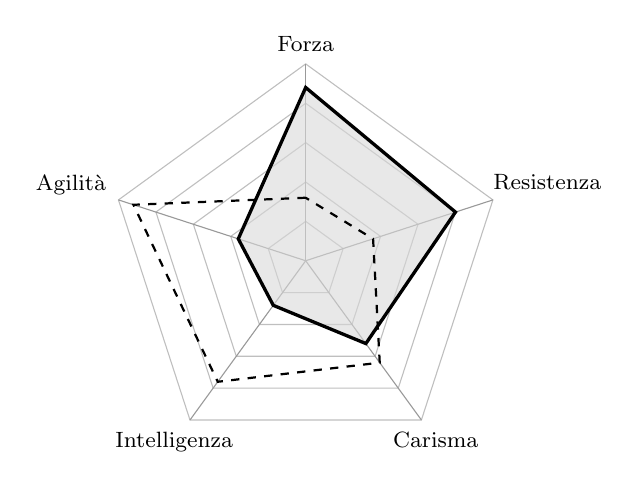
\begin{tikzpicture}[font=\footnotesize]
  \def\n{5}
  \foreach \r in {0.5,1,1.5,2,2.5} {
    \draw[black!25] (90:\r)
      \foreach \i in {1,...,4} { -- (90+\i*72:\r) } -- cycle;}
  \foreach \i/\lab in {0/Forza,1/Agilità,2/Intelligenza,3/Carisma,
                       4/Resistenza} {
    \draw[black!40] (0,0) -- (90+\i*72:2.5);
    \node[anchor=270+\i*72, inner sep=3pt] at (90+\i*72:2.55) {\lab};}
  \draw[very thick, fill=black!15, fill opacity=0.6]
    (90:2.2) -- (162:0.9) -- (234:0.7) -- (306:1.3) -- (18:2.0) -- cycle;
  \draw[thick, dashed]
    (90:0.8) -- (162:2.3) -- (234:1.9) -- (306:1.6) -- (18:0.9) -- cycle;
\end{tikzpicture}
\caption{Un grafico a radar con due profili di personaggio (valori
inventati): a colpo d'occhio si vede in quali categorie qualitative ciascuno
è spiccato.}
\label{fig:radar}
\end{figure}

\subsection{Il grafico a corde}

Nel \textbf{grafico a corde} (\emph{chord diagram}) ogni corda ha
un'\textbf{entrata} e un'\textbf{uscita}, indicata dalla punta della freccia.
L'esempio della slide mostra le \textbf{migrazioni globali} nel corso del
tempo.

\paragraph{Le relazioni tra sistemi.} Questo grafico è estremamente utile
quando si parla di \textbf{relazioni tra sistemi}. Si mettono a grafico tutti
i sistemi del gioco: il \emph{weather system}, il \emph{combat system}, gli
NPC, la vita sociale, e così via. Si mostra quanto sono collegati e in che
direzione (in un senso o in entrambi), e già a livello visivo si fa vedere
quanto, per esempio, il combattimento è collegato a tutto il resto, o quanto
un sistema invece è poco impattante e interessa relativamente meno. È un
altro modo per \textbf{mostrare} graficamente, invece di dover scrivere in
maniera esagerata, le relazioni tra i sistemi.

``Di grafici ce ne sono davvero tantissimi.'' Sta al designer imparare a
scegliere, come sempre, \emph{the right tool for the right job}; ``in questo
caso, \emph{the best tool for the right job}''.

% ---------------------------------------------------------------------
\section{La campagna di Russia in un grafico}
\label{sec:minard}

\subsection{Due avvertenze}

Per mostrare fin dove ci si può spingere, il docente ripropone un grafico già
intravisto, ``fichissimo, cioè per me è fichissimo'', con due avvertenze.
\begin{enumerate}
  \item Probabilmente lo si rivedrà al \textbf{terzo anno}, e verrà rifatta la
        stessa domanda: che cosa mostra? Ma il docente ``non cede di un
        passo'' e lo mostra lo stesso al primo anno, perché ``è troppo
        bello''. Al terzo anno, ``non mentite: noi lo sappiamo''.
  \item Il grafico è legato al \textbf{design}: fa parte di quel processo di
        \textbf{semplificazione} e di resa più grafica dei documenti di cui
        si sta parlando nelle lezioni di documentazione, e tornerà quando si
        parlerà di uno specifico tipo di documento, la ``summa'', il fine
        ultimo di questo processo.
\end{enumerate}

Il grafico viene attribuito a \textbf{Edward Tufte}, ``probabilmente il padre
delle infografiche'': ha dato i principi di base, alcuni dei quali sono
golden rules della documentazione (sezione~\ref{sec:golden-rules}), e sono
presi come base per fare UX e UI.\footnote{La mappa è in realtà opera
dell'ingegnere francese \textbf{Charles Joseph Minard} (1869). È stato Tufte,
in \emph{The Visual Display of Quantitative Information} (1983), a renderla
celebre, definendola probabilmente il miglior grafico statistico mai
disegnato.} Il docente darà poi il link a un talk che ne parla, ``uno dei
talk più belli che siano mai stati fatti sul design in generale, sul game
design in generale. A me ha aperto la mente.''

\subsection{Che cosa mostra?}

La regola del gioco: niente ``furia'', non si va a cercare che cos'è. Più ci
si spreme le meningi, più ritorno si avrà dopo. Si sa solo che è una
\textbf{variante del diagramma di Sankey}. E bisogna leggere il grafico, non i
testi (``sennò è troppo semplice'').

\begin{description}
  \item[Valerio] Potrebbe mostrare \textbf{scelte narrative} che proseguono
        con la storia. ``In questo caso no. Però è interessante: c'è un
        certo tipo di \textbf{progressione} in questo grafico.'' E, ammette il
        docente, ``ho mentito: sono due grafici'', uno sopra e uno sotto, che
        si legano tra loro.
  \item[Lorenzo] Sembra esserci una \textbf{correlazione} tra i due. La
        banda color ocra all'inizio è il 100\%; poi una parte si stacca, e
        nel tempo, procedendo, la quantità cambia, forse in un tempo comune
        alle due curve rappresentato da quella sotto. Nella banda nera si
        discrimina un'altra popolazione che si prende un'altra fetta. E
        quindi non sono percentuali ma \textbf{quantità}, perché nel tempo
        entrambe \textbf{diminuiscono}. ``Questo te lo confermo.'' Sembra uno
        strumento per analizzare più categorie e quantità correlate nel
        tempo. Il docente conferma la direzione: c'è una progressione,
        ``tra l'altro fisica''; la banda si rompe in quella nera, le
        quantità di entrambe diminuiscono, e c'è la correlazione con il
        grafico sotto, che è un \textbf{grafico a linea delle temperature}.
        Dalla classe si nota anche che la banda nera sembra ingrossarsi a
        spese dell'altra, e qualcuno azzarda un'ipotesi: petrolio bruciato e
        anidride carbonica emessa.
\end{description}

Il docente indica allora alcune linee sottili, ``con una forma che
sicuramente in vita vostra avete già visto''. Curve di livello? ``No, sono
troppo irregolari.'' Confini geografici? Una mappa delle temperature locali in
2D? Nessuno azzarda: sono \textbf{fiumi}.

\subsection{La risposta}

Il grafico mostra la quantità di uomini nell'\textbf{esercito di Napoleone
durante la campagna di Russia}, verso Mosca.
\begin{itemize}
  \item La banda chiara è la \textbf{marcia di andata}, quella nera la
        \textbf{ritirata}.
  \item La \textbf{larghezza} della banda è la grandezza dell'esercito.
  \item Durante la marcia alcuni se ne vanno: l'esercito si divide, alcuni
        tornano indietro, altri vanno avanti.
  \item In corrispondenza di un fiume si vede la banda assottigliarsi
        drasticamente: lì sono morti moltissimi uomini (``adesso io ci
        rido, ma non fa ridere'').
  \item Tutto in relazione alla \textbf{temperatura} in quei punti, che è il
        secondo grafico, sotto.
\end{itemize}

Per il docente ``è una figata'' perché, una volta letta la legenda,
\textbf{comunica immediatamente}, con un impatto grafico fortissimo, dove è
andato quell'esercito, che cosa ha vissuto, come si è piano piano non solo
separato ma anche \textbf{decimato} nel tempo: una campagna completamente
disastrosa. ``Con i grafici potete fare questa roba qua.''

\subsection{Dalle infografiche ai documenti}

In futuro si vedrà che lo stesso si può fare anche con la documentazione,
benché con i documenti di design sia veramente difficile: nella sua massima
espressione, \textbf{compressi in una singola pagina}. È il motivo per cui
Tufte è stato preso ad esempio e riadattato all'arte del documentare da
\textbf{Stone Librande}, il designer di \emph{Spore}, dei \emph{Sims} e di
altri titoli.\footnote{Nella trascrizione compare come ``Stanley Brandi''.
Il talk a cui il docente si riferisce è quasi certamente \emph{One-Page
Designs} di Stone Librande (GDC 2010), in cui la mappa di Minard e i principi
di Tufte sono il punto di partenza per i documenti di design di una sola
pagina.} Se ne riparlerà nella lezione di documentazione apposita. Non bisogna
raggiungere subito quel livello, ``perché è molto difficile, e non credo
nemmeno di esserci arrivato io''; ma il margine è tanto: \textbf{il tetto è
molto alto}. Si ragiona, si sperimenta, e si migliora nel tempo.

\paragraph{Approfondimento: Tufte nelle bibliografie di game design.} Tufte
compare nelle letture consigliate di entrambi i manuali del progetto.
Schell, in \emph{The Art of Game Design}, definisce \emph{The Visual Display of
Quantitative Information} ``la Bibbia (o almeno l'Antico Testamento) del
design delle interfacce grafiche'', e apre la sua lente della trasparenza
(\#62) con una citazione di Tufte: ``Per quanto bella sia la tua
interfaccia, sarebbe meglio se ce ne fosse di meno''. Brathwaite e Schreiber,
in \emph{Challenges for Game Designers}, consigliano \emph{Visual
Explanations}: per quanto si aderisca alle convenzioni di genere, sembra che
esistano solo uno o due modi di mostrare una barra della vita o il conteggio
delle munizioni; Tufte ``distrugge questa illusione'', mostrando molti modi
diversi di visualizzare un'informazione importante, con pregi e difetti di
ciascuno. È lo stesso messaggio della lezione: per ogni dato esiste un
grafico migliore degli altri, e trovarlo è parte del lavoro.

% ---------------------------------------------------------------------
\section{Principi per grafici migliori}
\label{sec:principi-grafici}

Ci sono comunque dei principi per migliorare, formattare e rendere più
visibili i dati di un grafico: le classiche regole della \textbf{Gestalt} e i
principi di design in generale. Cose che probabilmente si sanno già, ma è utile
ricordarle, e che si sono già cominciate ad applicare nella documentazione;
nei grafici le si può spingere ``all'esponenziale'', perché fare grafici è
``una pratica grafica, appunto''.
\begin{description}
  \item[Spazio negativo] Va sfruttato.
  \item[Scala] Ciò che è più grande impatta di più il lettore e viene
        percepito come più importante; ciò che è più piccolo, meno.
  \item[Gerarchia] L'ordine visivo delle informazioni.
  \item[Prossimità, forma, colore] Elementi vicini, della stessa forma o
        dello stesso colore vengono letti come un gruppo.
\end{description}

Al netto della ricerca (scoprire nuovi tipi di grafico, capire qual è il più
adatto) questa abilità si costruisce con l'\textbf{esperienza}: più grafici si
fanno, più si diventa abili, ``ancora di più rispetto alla documentazione
base, anche perché questo è documento''.

% ---------------------------------------------------------------------
\section{La matematica di base}
\label{sec:matematica-base}

\subsection{Quattro cose, da quinta elementare}

Non c'è tempo per un'altra pausa (``al massimo finiamo cinque minuti prima,
cosa che non è mai successa''), quindi si passa ai \emph{basic math
principles}. ``Qua siamo probabilmente in quinta elementare'': per chi non lo
sapesse non è un problema; le cose sono veramente quattro.

\subsection{La media}

La \textbf{media} (aritmetica) è la somma di tutti i numeri divisa per il
numero di elementi dell'insieme:
\[
  \bar{x} = \frac{x_1 + x_2 + \dots + x_n}{n} = \frac{1}{n}\sum_{i=1}^{n} x_i .
\]
``Su questo penso che nessuno abbia dei dubbi.''

\subsection{La media pesata}

Serve per alcuni framework o per alcuni calcoli in generale. Ci sono
\textbf{due modi} per farla.

\paragraph{Primo modo: pesi che sommano a uno.} Tutti i pesi sommati devono
dare \textbf{uno}, cioè il totale, il 100\%. Dati questi pesi, si
\textbf{moltiplica} ciascun valore per il rispettivo peso, ottenendo il valore
pesato, e poi si \textbf{somma}:
\[
  \bar{x}_w = \sum_{i=1}^{n} w_i\, x_i \qquad \text{con} \qquad
  \sum_{i=1}^{n} w_i = 1 .
\]

\paragraph{Secondo modo: pesi qualsiasi.} I pesi possono \textbf{non} dare il
100\%. Si moltiplica ciascun valore per il suo peso specifico, si sommano i
risultati, e la somma si divide per la \textbf{somma dei pesi}:
\[
  \bar{x}_w = \frac{\sum_{i=1}^{n} w_i\, x_i}{\sum_{i=1}^{n} w_i} .
\]
``Non è complessa, forse un passaggio in più.'' Il primo modo è un caso
particolare del secondo: se i pesi sommano a uno, il denominatore vale 1.

\paragraph{Un esempio.} Si vogliano confrontare due idee uscite dal
brainstorming dando un voto da 1 a 10 a tre criteri, con pesi diversi:
impatto (peso 3), costo contenuto (peso 2), coerenza con la visione
(peso 1). Un'idea con voti 8, 4 e 9 ha media semplice $(8+4+9)/3 = 7$, ma
media pesata
\[
  \frac{3\cdot 8 + 2\cdot 4 + 1\cdot 9}{3+2+1} = \frac{41}{6} \approx 6{,}83 .
\]
Con i pesi normalizzati ($3/6 = 0{,}5$; $2/6 \approx 0{,}33$;
$1/6 \approx 0{,}17$, che sommano a 1) si ottiene lo stesso risultato con il
primo modo. (L'esempio non è della lezione.)

\paragraph{Approfondimento: il valore atteso.} Schell (\emph{The Art of Game
Design}, capitolo~12) mostra uno degli usi più frequenti della media pesata
nel game design: il \textbf{valore atteso}, cioè la media di tutti i
risultati possibili di un'azione, pesati con la loro probabilità (pesi che,
come nel primo modo, sommano a uno). Se finendo su una casella verde si tira
un dado a sei facce e si ottengono altrettanti punti, il valore atteso è
$(1+2+3+4+5+6)/6 = 3{,}5$: è utile sapere che ogni volta, in media, si
guadagnano 3,5 punti. Con esiti non equiprobabili si pesa: tirando due dadi,
si vincono 5 dollari con un 7 o un 11 e se ne perde uno con qualsiasi altro
risultato. Le probabilità sono $6/36$ per il 7, $2/36$ per l'11 e $28/36$ per
il resto, quindi
\[
  \tfrac{6}{36}\cdot 5 + \tfrac{2}{36}\cdot 5 + \tfrac{28}{36}\cdot(-1)
  \approx 0{,}83 + 0{,}28 - 0{,}78 = 0{,}33 :
\]
alla lunga si vincono in media 33 centesimi a partita. Se vince solo il 7, il
valore atteso scende a zero (un gioco equo); se vince solo l'11, diventa
negativo ($-0{,}86$ circa). Schell ne fa una lente (\#35, \emph{The Lens of
Expected Value}): bilanciare un gioco passa spesso da conti di questo tipo.

\subsection{Le proporzioni}

L'ultima cosa è la \textbf{proporzione}: $a$ sta a $b$ come $c$ sta a $d$,
\[
  a : b = c : d ,
\]
dove $a$ e $d$ sono gli \textbf{estremi} e $b$ e $c$ i \textbf{medi}. La
proprietà fondamentale è che il prodotto dei medi è uguale al prodotto degli
estremi ($b \cdot c = a \cdot d$). Quindi:
\begin{description}
  \item[Incognita in un estremo] Si \textbf{moltiplicano i medi} e si divide
        per l'\textbf{estremo noto}. Esempio della lezione: in
        $100 : 35 = 20 : x$, i medi sono 35 e 20, l'estremo noto è 100:
        \[ x = \frac{35 \cdot 20}{100} = \frac{700}{100} = 7 . \]
        Verifica: 100 sta a 35 come 20 sta a 7.
  \item[Incognita in un medio] Si \textbf{moltiplicano gli estremi} e si
        divide per il \textbf{medio noto}. Esercizio della lezione: in
        $100 : 35 = x : 5$, gli estremi sono 100 e 5, il medio noto è 35. La
        classe risponde con il calcolo, ``500'', diviso 35:
        \[ x = \frac{100 \cdot 5}{35} = \frac{500}{35} \approx 14{,}3 , \]
        che il docente arrotonda a 14: 100 sta a 35 come (circa) 14 sta
        a 5.
\end{description}

``Avete tutte le informazioni basilari di matematica per sopravvivere alla
quinta elementare e al primo anno.''

\subsection{Che cosa verrà dopo}

Il discorso si complicherà al secondo anno, quando si parlerà di
\textbf{regressione lineare}: ma sono strumenti che servono per framework
specifici o per lavori specifici. Fare l'\textbf{economy designer} li
richiede, e anche un \textbf{data analyst} ha determinate competenze
matematiche; li si tratterà lì, punto per punto. Per ora interessa solo che
si ricordino queste quattro cose: semplici, ma ``una rinfrescata e averle lì
non vi fa male''.

% ---------------------------------------------------------------------
\section{Chiusura e prossimi appuntamenti}
\label{sec:chiusura-gd6}

La lezione è finita (``yes, abbiamo finito''), con un leggero margine di
anticipo. Il docente ricorda le scadenze:
\begin{itemize}
  \item il \textbf{production dictionary} per \textbf{lunedì 2}
        (sezione~\ref{sec:task-gd4});
  \item il \textbf{flowchart di Pac-Man} (o di \emph{Donkey Kong}) per
        \textbf{venerdì 6} (sezione~\ref{sec:task-gd6});
  \item l'altro task è già stato consegnato: il docente lo commenterà nel
        fine settimana o, al massimo, all'inizio della settimana successiva.
\end{itemize}

\paragraph{Leggere i commenti prima del 6.} Dopo che il docente avrà
commentato, bisogna \textbf{leggere i suoi commenti prima della lezione del
6}: in quella lezione si prenderà una pagina bianca e si comincerà a
documentare e a formattare la pagina insieme (sezione~\ref{sec:recap-documentazione}),
e prima di farlo è importante che il feedback ricevuto sia stato compreso.
Come detto l'altra volta, bisogna aspettare che il docente abbia commentato
tutto.

``Per lunedì portate il PC, perché Alessandro ne sarà sicuramente contento.''
I saluti sono di stagione: ``Buon Halloween! Buona festa dei morti!''

% ---------------------------------------------------------------------
\section*{Punti chiave del capitolo}
\addcontentsline{toc}{section}{Punti chiave del capitolo}

\begin{itemize}
  \item Nel \textbf{production dictionary} vanno i \textbf{nomi} unici o
        fraintendibili del gioco, spiegati in una o due righe (che cos'è una
        MT, che cos'è un tipo); il funzionamento profondo va nei documenti
        dedicati. Ordine alfabetico per leggibilità, ma le voci legate tra
        loro possono stare vicine; in ogni caso, \textbf{ordinato}.
  \item Nel brainstorming \textbf{nessuno viene fermato}, tutti parlano, si
        elenca tutto, si cercano background diversi. Un
        \textbf{facilitatore} (non un leader) fa sentire tutti ascoltati e
        tiene il brainstorming su uno scopo pratico. \textbf{Pause} e
        \textbf{cibo} riducono la tensione.
  \item Altre tecniche: circle, acting brainstorming, i \textbf{sei
        cappelli} di de Bono (partire dal verde; il nero è già giudizio),
        l'oggetto dal cappello, storyboard, domande, ``peggiore è, meglio
        è'', associative e \textbf{mind mapping}, il \textbf{TRIZ} (matrice
        di parametri, soluzione già nella cella, adatto a problemi
        fisici).
  \item Le regole di \textbf{Kawasaki} (make meaning, make mantra, next
        curve, DICEE, don't worry be crappy, hundred flowers, polarize,
        churn, niche, perfect your pitch) e lo \textbf{SCAMPER}. Il pitch si
        prova e riprova, ma \textbf{non si impara a memoria}.
  \item Dalle cento idee ad \textbf{almeno dieci}: \textbf{brainstorming
        matrix} impatto/effort, confronto, compromesso; contano anche la
        \textbf{motivazione} del team e la visione. Le idee vanno
        \textbf{distrutte}: se non si trova nessun difetto, c'è un problema.
  \item \textbf{KISS}: prototipare subito il cuore del gioco; muoversi,
        cambiare prospettiva, \textbf{rituali} che rompono la routine (il
        playtest del venerdì).
  \item Il \textbf{flowchart} è una rappresentazione grafica formalizzata di
        un processo; nasce nel software, e ai designer serve per IA,
        pipeline, game loop, sequenze di gameplay, player journey, UI.
        Serve a \textbf{mostrare invece di scrivere}.
  \item Regole: si legge \textbf{dall'alto in basso e da sinistra a
        destra}, nella direzione delle frecce; stesso livello, stessa
        gerarchia; il layout orizzontale evita il \textbf{wall of text}.
  \item Blocchi: \textbf{inizio/fine} (rettangolo arrotondato, obbligatori),
        \textbf{azione} (rettangolo), \textbf{decisione} (rombo, uscite
        sempre etichettate), \textbf{sotto-processo} (da spiegare in un altro
        flowchart), \textbf{input/output} (parallelogramma),
        \textbf{documento}.
  \item In un sistema o un loop di gioco il flusso \textbf{deve chiudersi o
        tornare indietro}: nessun ramo nel nulla. Le regole prima si
        imparano, poi si piegano (Oxenfree, il gioco di carte, Machinations,
        il behavior tree).
  \item Task: il \textbf{flowchart completo di Pac-Man} (Daniele:
        \emph{Donkey Kong}), come immagine leggibile e commentabile,
        esportata al 300--500\%, per venerdì 6.
  \item Grafici: \textbf{linea} per l'evoluzione continua e le previsioni,
        \textbf{gradini} per i salti discreti e le progressioni; barre e
        colonne (con legenda prima), istogrammi, torta e ciambella, aree,
        clustering; poi treemap, sunburst, \textbf{radar}, \textbf{corde}
        (relazioni tra sistemi) e la mappa di Minard resa celebre da Tufte.
        Il tetto è altissimo: fino ai documenti di una pagina di Librande.
  \item Matematica di base: \textbf{media}, \textbf{media pesata} (pesi che
        sommano a uno, oppure divisione per la somma dei pesi; il valore
        atteso ne è un caso), \textbf{proporzioni} (medi per medi, estremi
        per estremi).
\end{itemize}
